\documentclass{scrartcl}
\usepackage{lipsum}
%%\usepackage[french]{babel}
%%\usepackage[ngerman]{babel}

%% Choose default font for the document
%% Warning : only ONE of the following should be enabled
\usepackage{kpfonts}
%%\usepackage{libertine}
\usepackage[table]{xcolor}
%% The following chose the default language for the document and
%% use the default typography rules for the chosen language.
\usepackage{polyglossia}
\setdefaultlanguage{english}
%% \setdefaultlanguage{german}
%%\setdefaultlanguage{french}
\usepackage{float}
\usepackage[toc,page]{appendix}
\usepackage[backend=biber, style=ieee]{biblatex}
\addbibresource{bibliothek.bib}
\usepackage[export]{adjustbox}
\usepackage{menukeys}
\usepackage{abstract}
\usepackage{pdfpages}
\usepackage{hyperref}
\usepackage{graphicx}
\usepackage{listings}
\lstset{language=C,
    basicstyle=\ttfamily,
    keywordstyle=\bfseries,
    showstringspaces=false,
    morekeywords={include, printf, interface}
}
\title{Anastais Project Documentation}
\date{September 2, 2020}
\author{Dominik Meister, Dennis Neufeld}

\begin{document}
\maketitle

\pagenumbering{gobble}

\clearpage
\pagenumbering{roman}
\tableofcontents
\listoffigures
\clearpage
\pagenumbering{arabic}
\section{Introduction}

Keys are used to encrypt high sensitive personal data and therefore
they must be kept safely.  Secure storage of private keys is known to
be a difficult problem --- especially for end-users with limited
skills in system administration and insufficiently redundant hardware.
A central objective for any solution is that only the legitimated
owner of a key must have the possibility to recover a lost key.

But how can one create a confidential backup of a key? It certainly
makes no sense to encrypt a key with a different password and then use
the result as a backup. After all, this merely shifts the problem from
the original key to the password, which is basically yet another key.
So simply encrypting the key is not helpful.  But without encryption,
any copy of a key increases availability, but also the risk of the
key's confidentiality being compromised.

Most people have difficulties memorizing a high-entropy
passphrase. Hence, existing key management ``solutions'' often reduce
the problem of memorizing one or more high-entropy passphrases or keys
to memorizing a single low-entropy passphrase. This is not a good
solution, as the low-entropy passphrase undermines security.

In this thesis, we describe a software solution for the described
problem using secret splitting.  We call our solution ``Anastasis'',
which is a medical term for the prognosis of full recovery.  We will
call the information that Anastasis allows the user to recover their
{\em core secret}.

\subsection{Principles}

For Anastasis we have following design objectives, in order of importance:

\begin{enumerate}
 \item Anastasis must be Free Software\footnote{\url{https://www.fsf.org/}}. Everyone must have the right to
   run the program, study the source code, make modifications and share
   their modifications with others.
 \item Anastasis must not rely on the trustworthiness of individual providers.
   It must be possible to use Anastasis safely, even if a subset of the
   providers is malicious. Anastasis must minimize the amount of information
   exposed to providers and the network.
 \item Anastasis must put the user in control: They get to decide which
   providers to use, and which combinations of authentication steps will
   be required to restore their core secret. The core secret always remains exclusively
   under the user's control, even during recovery.
 \item Anastasis must be economical viable to operate. This implies usability
   and efficiency of the system.
 \item Anastasis must support a diverse range of use cases.
\end{enumerate}


\subsection{Approach}

\subsubsection*{Secret sharing and recovery}

Our approach to solve the problem of key recovery is to let the user
split their core secret across multiple escrow providers (see
Figure~\ref{fig:system_arch2}). To recover their core secret, the user has to
authorize key the recovery, usually by passing an authentication check
which they configured for the respective provider.

After successful authentication the user receives the secret shares
and is able to reassemble their core secret locally on their computer.

\begin{figure}[H]
\centering
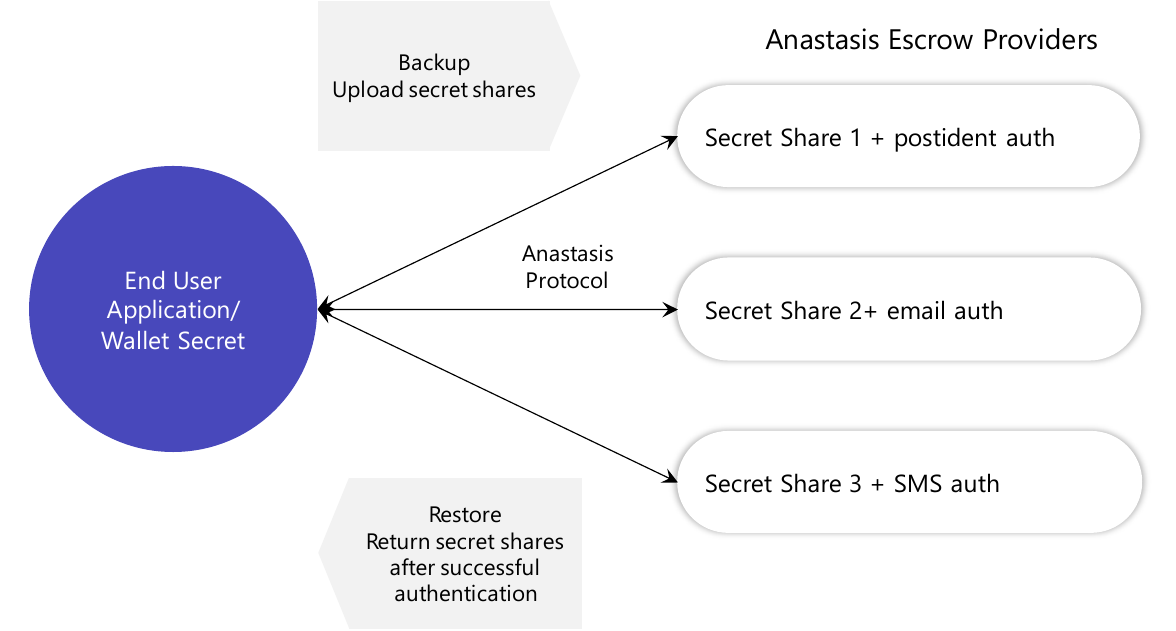
\includegraphics[scale=0.33]{images/system-architecture_2.png}
\caption{System architecture}
\label{fig:system_arch2}
\end{figure}

\subsubsection*{Derive user identifier}

Every person has some hard to guess, semi-private and unforgettable
inherent attributes such as name and passport number, social security
number or AHV~\cite{jerome2015} number (in Switzerland).  We use those attributes to
improve the security and privacy provided by Anastasis.  Basically,
these attributes serve as weak key material, raising the bar for
attackers without the availability disadvantages of passphrases ---
which users may forget.  Anastasis derives a ``user identifier'' from
such a set of unforgettable attributes (see Figure~\ref{fig:user_id}).

\begin{figure}[H]
\centering
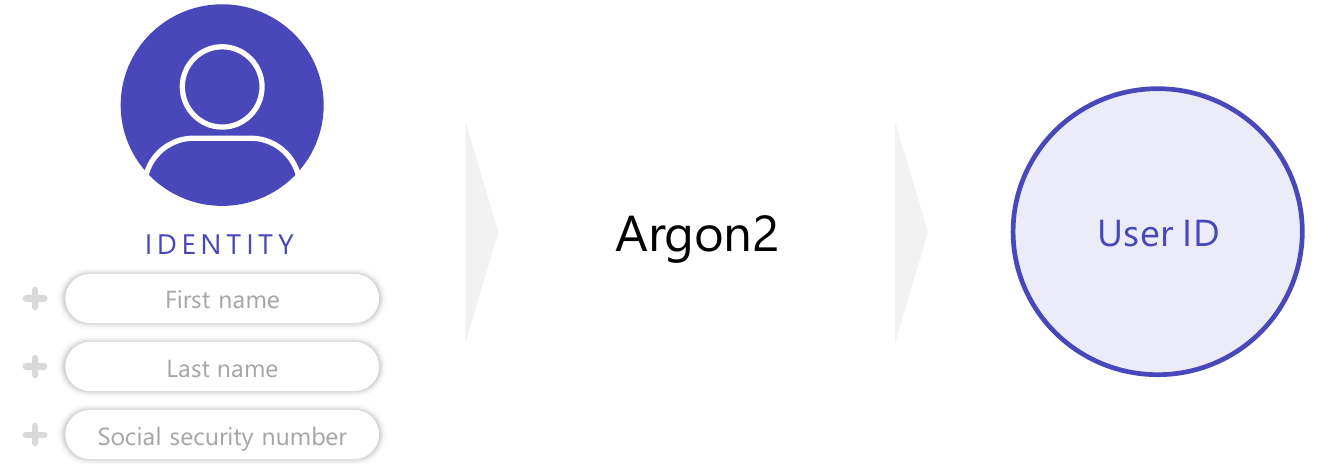
\includegraphics[scale=0.3]{images/user_id.png}
\caption{Derivation of a user identifier}
\label{fig:user_id}
\end{figure}

\subsubsection*{Encrypt and encrypt and encrypt}

Anastasis uses several layers of encryption. First, the user's core
secret is encrypted with a master key. The master key is encrypted
with various policy keys. The policy keys are derived from various
secrets which are encrypted and distributed across various providers
together with information about the desired recovery authorization
procedure. This last encryption is done based on keys derived from the
user identity.  These many layers of encryption are designed to
distribute trust and to minimize or delay information disclosure.

\subsubsection*{Private payments are integrated}

The Anastasis protocol includes provisions for privacy-preserving
electronic payments to the service providers, as well as resource
limitations to protect service providers against resource exhaustion
attacks.  This ensures that it should be possible to operate the
service commercially.


\subsection{Use cases}

There are several applications which are in need of a key escrow
system like Anastasis. Some of them shall be introduced in this
section.

\subsubsection{Encrypted email communication}

For email encryption using Pretty Good Privacy
(PGP)~\cite{garfinkel1995} users need a private key which is typically
stored on the device running PGP.  PGP uses a ``Web of trust'' to
establish the authenticity of keys.

Pretty Easy privacy (short p\equiv p) is ``a cyber security solution
which protects the confidentiality and reliability of communications
for citizens, for public offices and for
enterprises''~\cite{pepdoc}. It secures communication via email by
providing end-to-end encryption similar to PGP.  A major difference is
that p\equiv p uses opportunistic encryption and so-called trustwords
to establish authenticity to avoid usability and privacy problems
associated with the ``Web of trust''~\cite{caronni2000}.

The impact of losing control over the private key is similar in both
systems:

\begin{itemize}
  \item If the private key becomes unavailable, all emails which were
encrypted to that key become unreadable. Furthermore, the user would
likely need to rebuild their ``Web of trust''.
  \item If the private key is
disclosed to an adversary, they might be able to decrypt that user's
encrypted emails -- which may go back years and could include highly
sensitive information.  An adversary could also use the private key
to send cryptographically signed emails pretending to be the user.
\end{itemize}


\subsubsection{Digital currencies and payment solutions}

Another application relying on a core secret are cryptocurrencies like
Bitcoin. Each user of Bitcoin needs an electronic wallet which stores
and protects the private keys of the user. Those private keys
legitimate its owners to spend the bitcoins corresponding to the
keys.~\cite{LLLW*2017}

Losing Bitcoin wallet keys means losing all of the corresponding
Bitcoins.  The reader may be familiar with stories from the mass media
about people who claim to have lost their key to their electronic
wallet and therefore huge sums of
cryptocurrency~\cite{millions_lost}. Backup systems are essential to
avoid such cases.

The following graphic illustrates the keys used in Bitcoin
wallets. In this case, the core secret Anastasis would store
is the ``master key'' $m$:

\begin{figure}[H]
	\centering
	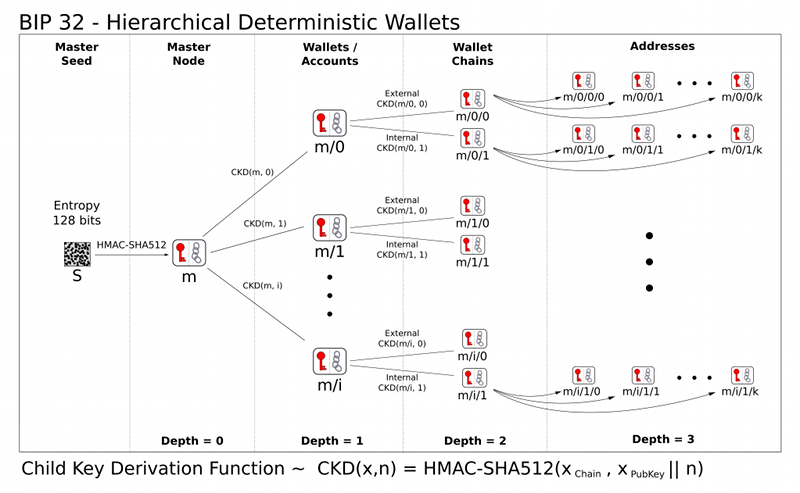
\includegraphics[scale=3.5]{images/bitcoin-keys.png}
	\caption[Master key in Bitcoin wallets]{Master key in Bitcoin wallets (from~\cite{bitcoin-keys})}
	\label{fig:bitcoin_keys}
\end{figure}

GNU Taler\footnote{\url{https://taler.net/de/}} is a new electronic instant payment system for
privacy-friendly online transactions. The GNU Taler digital wallets are
storing electronic coins, and backups are protected with a key.
Losing the backup key means losing all the money stored in the wallet,
as well as the transaction history kept in the wallet.

The European Central Bank (ECB) informally informed Taler Systems SA
about the requirement for electronic wallets denominated in Euros to
support password-less data recovery to ensure users would not loose
their electronic funds if their device were to be damaged or lost.

This was the key impulse which motivated us to create Anastasis,
with the goal of enabling recovery of GNU Taler's backup keys via
Anastasis.


\subsubsection{Password managers}

To avoid using low-entropy passwords and password reuse, some people
use software password managers like
KeePass\footnote{\url{https://keepass.info/}}. Such password managers
relieve you of the burden of remembering many passwords and in most
cases allow the generation of high-entropy passwords.

The user only has to remember the password for the password
manager. However, as discussed before, this is still a major problem:
\begin{itemize}
  \item On the one hand, users could use an insecure, easy to
remember password. In this case, an adversary gaining control
over the password manager's database could break into all systems
secured by keys managed by the password manager.
\item On the other hand, users could use a complex, high-entropy
  passphrase.  However, if that passphrase is forgotten, users
  face the loss of all passwords and thus also all online
  services that the password manager controlled for them.
\end{itemize}

Anastasis can be used to enable recovery of strong passphrases,
such as those that should be used to secure password managers.


\subsubsection{Hard drive encryption}

Data at rest is often protected using (full) drive encryption, for
example using software like
LUKS\footnote{\url{https://guardianproject.info/archive/luks/}}.  For
encryption and decryption of the drive a combination of key files,
passphrases and Trusted Platform Modules (TPMs)~\cite{bajikar2002} are
used.

Anastasis can be used to backup and restore such key files or
passphrases.


\section{Related work}

This chapter explains some important cryptographic functions and which
are used in Anastasis or related to our work. We also describe issues
with existing solutions in this domain.

\subsection{Cryptographic primitives}

\subsubsection{Pseudo-randomness}

A pseudo random generator (PRG) is an algorithm producing an infinite
sequence of bits for which there is no efficient algorithm to
distinguish it from a truly random sequence~\cite{vadhan2012}. The
algorithm ``takes as input a short, perfectly random
seed''~\cite{vadhan2012} which determines the output value.\\

A pseudo random function (PRF) is a deterministic function which
output is finite and indistinguishable from a true random
function.~\cite{nielsen2002} PRFs can be constructed using
PRGs.~\cite{GGM1986}

\subsubsection{Hash function}

Hash functions "compress a string of arbitrary length to a string of
fixed length [...]"~\cite{Preneel1999}. The output of a hash function
often is called a "hash".  Hash functions in general should be very
fast to compute. Cryptographic hash functions need to fulfil
additional security requirements which are

\begin{itemize}
 \item (first) pre-image resistance,
 \item second pre-image resistance,
 \item collision resistance,
 \item pseudo randomness, and the
 \item avalanche effect.
\end{itemize}

Pre-image resistance, also called the ``one way property'', means that
for a given hash function $H$ and a hash value $H(x)$, it is
computationally infeasible to find $x$.~\cite{SG2012} For example,
since in Anastasis we derive the key to encrypt the personal details
required for user authentication (e.g. the mobile phone number for
authentication via SMS) using functions based on hash functions (see
HKDF), it is very important that you cannot derive the corresponding
input values from the key.

The second pre-image resistance is described by following: For a given
hash function $H$ and a hash value $H(x)$, it is computationally
infeasible to find $x$ and $x'$ such that $H(x) = H(x')$ and $x \not=
x'$.~\cite{SG2012} In Anastasis hash functions also are involved in
signing our so called recovery document. Hence an attacker should not
be able to create a malicious recovery document with the same hash
value as the original one.

The definition of collision resistance slightly differs from the
second pre-image resistance: For a given hash function $H$, it is
computationally infeasible to find a pair $x, y$ such that $H(x) =
H(y)$ \cite{SG2012}.
%CG: the text below does NOT related to collision resistance!
%As we are using HKDFs for deriving keys in
%Anastasis, an attacker should not be able to find some other input
%values also leading to the same keys we use.
Anastasis does not rely upon collision resistance in its use of hash
functions. % CG: at least no case comes to mind for me right now...

A cryptographic hash function should also behave as a pseudo random
function. This means that although a hash function is purely
deterministic, the output must not be predictable.

The avalanche effect describes the property of an algorithm that
causes a significant change of the output value, usually a bit
flipping of more than half the output is desired, if the input is
changed slightly (for example, flipping a single bit).~\cite{RK2011}
The more bits are flipping in the output value the higher the entropy
of the randomness of the hash function.

There are many applications for cryptographic hash functions. For
example, you can store the hash value of a passphrase instead of the
passphrase itself in a computer to protect the passphrase. Another
important application is verification of message integrity: Before and
after transmission of a message one can calculate the hash values of
it and compare hashes later to determine if the message changed during
transmission.

In Anastasis we use SHA-512~\cite{GJW2011} for fast hash functions.

\subsubsection{HMAC}

When it comes to integrity of messages during communication of two
parties over an insecure channel Keyed-Hash Message Authentication
Codes (HMAC) are used as check values. An HMAC function is based on a
hash function and takes two arguments, a key $K$ and a message $M$:

$HMAC_{K}(M) = H(K \oplus opad,H(K \oplus ipad, M))$ with "ipad" and
"opad" being constants which fill up the key $K$ to the blocksize of
the hash function~\cite{BCK1996}. The blocksize of a modern hash
function like SHA-512 is 64 bytes.

\subsubsection{HKDF}

A HKDF is a key derivation function (KDF) based on HMAC. A KDF ``is a
basic and essential component of cryptographic systems: Its goal is
to take a source of initial keying material, usually containing some
good amount of randomness, but not distributed uniformly or for which
an attacker has some partial knowledge, and derive from it one or more
cryptographically strong secret keys''~\cite{krawczyk2010}.

Anastasis uses HKDFs based on SHA-512 to derive symmetric keys for
encryption.

\subsubsection{Argon2}

Hash functions like SHA-512 are designed to be very fast. Therefore
passwords being stored using this kind of hash are vulnerable to
dictionary attacks with new hardware architectures like
FPGAs~\cite{trimberger2012} and dedicated ASIC~\cite{madurawe2006}
modules. But those architectures ``experience difficulties when
operating on large amount of memory''~\cite{BDK2016}.

In contrast to standard hash functions there are functions designed to
be memory-hard. Argon2 is such a memory-hard function that won the
Password Hashing Competition in 2015. It minimizes time-memory
tradeoff~\cite{stamp2003} and thus maximizes the costs to implement an
ASIC for given CPU computing time~\cite{BDK2016}. Aside from the fact
that Argon2 makes dictionary attacks much harder, Argon2 can be used
for another feature too: Memory-hard schemes like Argon2 are very
useful for key derivation from low-entropy sources~\cite{BDK2016}.

Argon2 is used in Anastasis to derive an identifier for the user from
the user's attributes, which serve as low-entropy inputs.


\subsection{Secret sharing}

Secret splitting, also known as secret sharing, is a technique for
distributing a secret amongst multiple recipients. This is achieved by
assigning a share of the secret to each recipient. By combining a
sufficient number of those shares, it is possible to reconstruct the
secret.  In a secret sharing theme the recipients of a share often are
called \textit{players}. The figure who gives a share of the secret to
the players is called \textit{dealer}.

In Anastasis the user is the trusted dealer who splits the secret and
also reconstructs it.

\subsubsection{Shamir's secret sharing} \label{sec:rel:shamir}

The algorithm ``Shamir's secret sharing'' is probably the most well
known secret sharing scheme. It ``divide[s] data D into n pieces in
such a way that D is easily reconstructible from any k pieces, but
even complete knowledge of $k - 1$ pieces reveals absolutely no
information about D''~\cite{shamir_sharing}.

Shamir’s simple secret sharing scheme has two key limitations. First,
it requires a trusted dealer who initially generates the secret to be
distributed, and second the shares are not verifiable during
reconstruction. Therefore, malicious shareholders could submit corrupt
shares to prevent the system from reconstructing the secret --- without
these corrupt shareholders being detectable as malicious. Furthermore,
the dealer distributing the shares could be corrupt and distribute
some inconsistent shares to the others. Also, in some scenarios the
dealer cannot be trusted with the knowledge of the original core
secret.

Additionally, Shamir's secret sharing is inflexible because it is a
simple $k$-out-of-$n$ threshold scheme.  While this makes the scheme
reasonably efficient even for big values of $n$, efficiency with
respect to a large number of escrow providers and authorization
procedures is not important for Anastasis: it is already difficult to
conceive users providing more than a handful of authentication methods
(Section~\ref{sec:rel:authentication} describes common choices.)

For Anastasis, we thus decided to opt for more flexible approach that
allows complex policies for recovery authorization, instead of only
$k$-out-of-$n$. Each user of Anastasis is also able to decide which
combinations of \textit{players}, which in case of Anastasis are the 
escrow providers, shall be permitted.

\subsubsection{Verifiable secret sharing}

Verifiability can be achieved by using so called commitment schemes
like the Pederson commitment. It allows ``to distribute a secret to n
persons such that each person can verify that he has received correct
information about the secret without talking with other
persons''~\cite{pedersen_sharing_0}. In his paper ``A Practical Scheme
for Non-interactive Verifiable Secret
Sharing''~\cite{feldman_sharing}, Paul Feldman combines the two
schemes Shamir Secret Sharing and Pederson commitment. His algorithm
for verifiable secret sharing (VSS), allows each recipient to
verify the correctness of their share. But like in the Shamir Secret
Sharing scheme, the dealer in the VSS scheme
also can't be trusted with the knowledge of the original core secret.

Because in Anastasis each user can act as their own trusted dealer,
the shares must not be verified and therefore Anastasis do not need
any form of VSS.

\subsubsection{Distributed key generation}

Distributed key generation (DKG) algorithms solve the problem of
needing a trustworthy dealer by instead relying on a threshold of
honest persons for key generation. Contrary to the above-mentioned
schemes, in distributed key generation algorithms every participant is
involved in key generation.  The Pederson DKG is such ``a secret
sharing scheme without a mutually trusted
authority''~\cite{pedersen_sharing_5.2}. Basically, this DKG works as
follows: First, each involved party generates a pre-secret and
distributes it to all parties using the verifiable secret sharing
scheme of Feldman.  Afterwards, each party recombines the received
shares, including its own pre-secret, to a share of the main
secret. The main secret can be reconstructed by summing up each
recombination of the shared pre-secrets.

Because in Anastasis each user can act as their own trusted dealer, we
also do not worry about the dealer learning the user's key and hence
Anastasis do not need any form of DKG.

\subsection{Authentication} \label{sec:rel:authentication}

To build a secure authentication procedure, today multi-factor
authentication is the standard~\cite{multifactor_authentication}. A
single authentication method by itself is usually vulnerable.
Multi-factor authentication combines multiple authentication
procedures to enhance the security of the system.

During procedure of some authentication methods a so called token is 
sent to the user. The user than has to provide the token to authorize.\\
The token should be a randomly generated passphrase which has at 
least 128 bits of entropy. It is best practice for a token to have an 
expiration time, although this is not relevant for security of Anastasis.\\

Anastasis is designed to use a wide range of authentication methods to
authenticate its users. Even though the user in Anastasis is free to
specify only one authentication method, we strongly recommend the use
of multi-factor authentication, typically using different
authentication methods at different providers.

A short overview of common authentication methods and issues with
each of them is presented here.

\subsubsection{Password authentication}

Password authentication is probably the most widely used
authentication procedure. But as studies show the procedure has its
drawbacks~\cite{authentication_methods_review}. For example the
handling of the passwords, like storage or transmission, often is done
poorly. Another problem is that the user must remember his
password. Therefore the password is limited to the capabilities of the
user to remember it. Thus people tend to use passwords with low
entropy. Those passwords are vulnerable to brute force attacks or
dictionary attacks. Another problem using passwords is the possibility
of replay attacks: A password can be stolen by an eavesdropper during
online transmission and used by the attacker.

Because passwords can be forgotten, we do not recommend using this
method for provider-authentication in Anastasis. Users could easily
add a passwords into their set of ``invariant'' attributes used to
derive the identity key, and then would automatically obtain all of
the possible benefits (and drawbacks) from using a password.
Specifically, they must make sure that the password cannot be
forgotten, even if it means that the password has low entropy.

\subsubsection{Secure question}

Similar to password authentication the use of an authentication method
based on a secure question requires the user to remember the correct
answer to a specific question. The difference here is that the
question provides a context that helps the user to remember the answer
and the user does not necessarily need to memorize something
new~\cite{just2004}.

There are several variations to implement authentication using a
secure question:

\begin{itemize}
 \item The questions and answers are predefined.
 \item Just the questions are predefined.
 \item The user is free to create custom questions and answers.
\end{itemize}

The first option is the easiest one. But predefining the answers has
the disadvantage being impersonal and inflexible. The questions must
inevitably be general, which may allow an attacker to obtain answers
by collecting public information about the victim, or even simply
solving the challenge by brute-forcing trying all possible choices.
Therefore the first option is not ideal.

The second option is more applicable but has some drawbacks, too. For
example there may be questions whose answers have multiple syntactic
representations (for example, ``St.'' versus
``Street'')~\cite{just2004}. Another problem could be a question whose
answer may change over time. Asking for the favourite actor for
example could be problematic. In addition, there is a challenge to
define questions for all kind of people. Some people for example could
not answer to the question, what the name of their pet is, because
they do not have one.

In case of the third option, we have all of the issues of the second
one, but additionally there is the difficulty for the user to ask
creative questions. A good question should only be answerable by the
user. Also, it would be perfect to have the attacker on the wrong
track by using ambiguous questions with word plays the adversary
cannot easily comprehend.

Authentication using a secure question requires checking the validity
of an answer that may include private personal information.
Consequently, Anastasis does not store the answers of secure questions
in cleartext. Instead, Anastasis only stores the hash value of a
(salted) answer.  Thus the user only has to provide the hash value of
the answer and not disclose the answer itself.

\subsubsection{SMS authentication}

Another way to authenticate users that have a mobile phone is to use
SMS authentication. The most popular use case is the so called Mobile
TAN used to authorize online banking transactions. A Mobile TAN is an
SMS based One-Time Password (OTP), short SMS OTP. SMS OTPs ``were
introduced to counter phishing and other attacks against
authentication and authorization of Internet
services''~\cite{MBSS2013}.

However, SMS authentication is not very secure, as it relies on the
security of the mobile network, which has various
vulnerabilities~\cite{rieck_detection}. There are also specialized
mobile trojans which are used to eavesdrop on these messages directly
on the user's mobile device.

While likely not as sensitive as answers to security questions, we
still consider user's phone numbers as private information that
deserves protection.  Naturally, a service authenticating the user
needs the phone number to send a message to the user during SMS
authentication.

Hence, Anastasis providers have to learn the phone number during SMS
authentication.  However, we can use cryptography to ensure that the
provider only gets the keys to decrypt the phone number when the
authentication process is started by the user as part of a recovery
operation. Thus, a compromise of the provider's database would not
directly reveal the phone numbers to the attacker.


\subsubsection{E-mail authentication}

Authentication by email is similar to SMS authentication. Here,
the user receives a token by email and has to provide it during the
authentication process.

It is important that the email should not already contain the
requested information, so in the case of Anastasis the keyshare.  This
is because the SMTP protocol used for email offers no hard security
assurances. In particular, the email is likely to be stored for a
indefinite period in the user's mailbox, which could be easily
compromised and read by a mailbox provider.~\cite{emailauthowasp}

Like with SMS authentication, Anastasis also encrypts the email
addresses when they are stored at the provider.  The user has to
provide the corresponding decryption key to the server during
the authentication process.


\subsubsection{VideoIdent}

VideoIdent uses a video chat to verify the identity of a user. The
user needs to show their face using a camera to an employee of the
VideoIdent service. The service then verifies the identity of the user
by comparing the video stream to a picture of the
user~\cite{pohlmann2017}.

Prerequisites for error-free identification are a video camera with
good video quality and a high-resolution image of the user on which
the face can be clearly seen. The user should also not change their
outward appearance too much over time. For example, growing or
trimming a beard could lead to the VideoIdent-service employee not
being able to recognise a user with sufficient confidence.

For an attacker who looks similar to the user, there is a chance that
the employee incorrectly confirms the identification.

%CG: that's IMO then e-mail based verification, should not mix
%    the two: this is basically multi-factor, so I'd leave it out here!
%Therefore, some interaction of the user is needed like for example
%telling the employee a short code which has been sent right before to
%the user by mail.

In Anastasis, pictures of users for VideoIdent authentication are
considered private information stored encrypted at the providers.
During the authentication process, the user has to provide the correct
key for decryption to the service.

\subsubsection{PostIdent}

It is also possible to sent a verification code to the user by
physical mail. A major drawback of this authentication method is
that it has high latency, and there is also the possibility that
physical mail gets intercepted or lost during transmission.

Anastasis providers using PostIndent would not store the address of
their users in cleartext. Instead the address is encrypted by the user
and the provider would receive the key to decrypt the address only
during the authentication process.

\subsubsection{Biometric authentication}

Another way of authenticating is the biometric
approach~\cite{biometric_auth}. Biometric authentication is based on
``something you are'', like your iris or your fingerprint.

Biometric authentication is highly problematic because the attributes
are invariant and frequently shared involuntarily.  Unlike passphrases
or phone numbers, users cannot change their genome or fingerprint in
case their private biometric information is exposed.  Furthermore,
there are credible threats against biometric authentication, in
paritcular there are documented inexpensive attacks against
fingerprint and iris scan authentication. For example, a member of the
German CCC e.V. was able to generate replicas from Angela Merkel's
iris and Ursula von der Leyen's fingerprint~\cite{ccc_merkel}.



\subsection{Existing solutions for key recovery}

This section introduces some existing solutions for key recovery and
why they are problematic.


\subsubsection{Coinbase}

Coinbase\footnote{\url{https://www.coinbase.com/}} is a global digital
asset exchange company, providing a venue to buy and sell digital
currencies. Coinbase also uses wallets secured with private keys. To
recover this private key the user has to provide a 12 words recovery
phrase.

Coinbase offers a solution to securely deposit this recovery phrase
onto the users Google Drive or iCloud.~\cite{coinbase} The security
here lies within the Google or iCloud account and another password
used to encrypt the security phrase. The problem here is that this
approach undermines confidentiality, as encrypting a strong key with a
weak key simply reduces the security to that of the weaker key.

\subsubsection{MIDATA}

MIDATA is a project that aims to give patients back control over their
medical data and to enable them to share their data only with those
they trust.\footnote{\url{https://www.midata.coop/}} In case a patient
lost their device with the MIDATA-application and also forgot their
MIDATA password, MIDATA provides a key recovery system using the
Shamir Secret Sharing scheme (as described in
Section~\ref{sec:rel:shamir}).

In their case, a few ``persons working at MIDATA have generated a
public-private key pair (Recovery key) on their own computer. They
keep the private recovery key for themselves and never share it. The
public keys are made public so that the apps can also access
them''~\cite{midata}. Using Shamir's Secret Sharing the MIDATA
application splits the user's app private key into 5 parts which are
encrypted with one of the published recovery keys. The encrypted parts
are then stored into the MIDATA server. During the recovery process at
least two of the 5 parts need to be decrypted by the persons owning
the private key part of the recovery key. ``The decrypted parts are
sent to the server and {\em the server} may now reconstruct the app
private key if enough parts of the key have been
decrypted''~\cite{midata}. (Emphasis ours.)

The security of MIDATA as described in ``Patient empowerment in IoT
for eHealth - How to deal with lost keys?''~\cite{midata} is broken in
three ways:

\begin{enumerate}
 \item The password is reconstructed at {\em the server}, not on the
   patients device. An administrator of the server could thus
   access the recovered password at that time.  It would be better
   to reconstruct the password only on the patients device.
 \item It is not clear which authentication methods the persons
   working for MIDATA use for their decisions and activities regarding
   the key recovery. The business process used here could be
   vulnerable, and it is not clear whether multi-factor authentication
   is used. As a result, we worry that it may be possible for an attacker
   to successfully use social engineering via email (or other means)
   to illegitimately trigger a recovery process.
 \item The MIDATA system also does not offer any trust agility~\cite{marlinspike2011}.
   The user is forced to accept the 2-out-of-5 rule with trustees
   provided by MIDATA.
\end{enumerate}


\section{Design} \label{chap:design}

Anastasis is a service that allows the user to securely deposit a {\em core
secret} with an open set of escrow providers and recover it if the
secret is lost. The core secret itself is protected from the escrow
providers by encrypting it with a {\em master key}. The main objective of
Anastasis is to ensure that the user can reliably recover the core
secret, while making this difficult for everyone else. Furthermore, Anastasis
supports situations where the user is unable to reliably remember any secret
with sufficiently high entropy, so Anastasis does not simply encrypt using some
other key material in exclusive possession of the user.

To uniquely identify users and to provide a first layer of protection,
an “unforgettable” identifier is used. This identifier should be
difficult to guess for anybody but the user. However, the identifier
is not expected to have sufficient entropy or secrecy to be
cryptographically secure. Examples for such an identifier would be a
concatenation of the full name of the user and their social security
or passport number(s). For Swiss citizens, the AHV number could also
be used.

\subsection{Overview}

The Figure~\ref{fig:legend_keys_anastasis} shows the legend for the
illustration of the Anastasis key usage shown in Figure~\ref{fig:keys_anastasis}
on page~\pageref{fig:keys_anastasis} and in
Figure~\ref{fig:truth_keys} on page~\pageref{fig:truth_keys}.
The Figure~\ref{fig:keys_anastasis} gives an overview of the keys used in Anastasis. It also shows how they are created and used.
Figure~\ref{fig:truth_keys} shows how the keys to sign the (encrypted) truth
data used during authentication are generated. The truth seed(s) used in
Figure~\ref{fig:truth_keys} are part of the recovery document.
\newline
\begin{figure}[H]
	\centering
	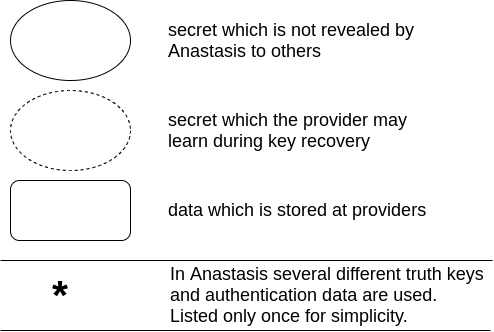
\includegraphics[scale=0.48]{images/legend_keys_anastasis.png}
	\caption{Legend of Figure~\ref{fig:keys_anastasis}} on page~\pageref{fig:keys_anastasis}
	\label{fig:legend_keys_anastasis}
\end{figure}

\begin{figure}[H]
	\centering
	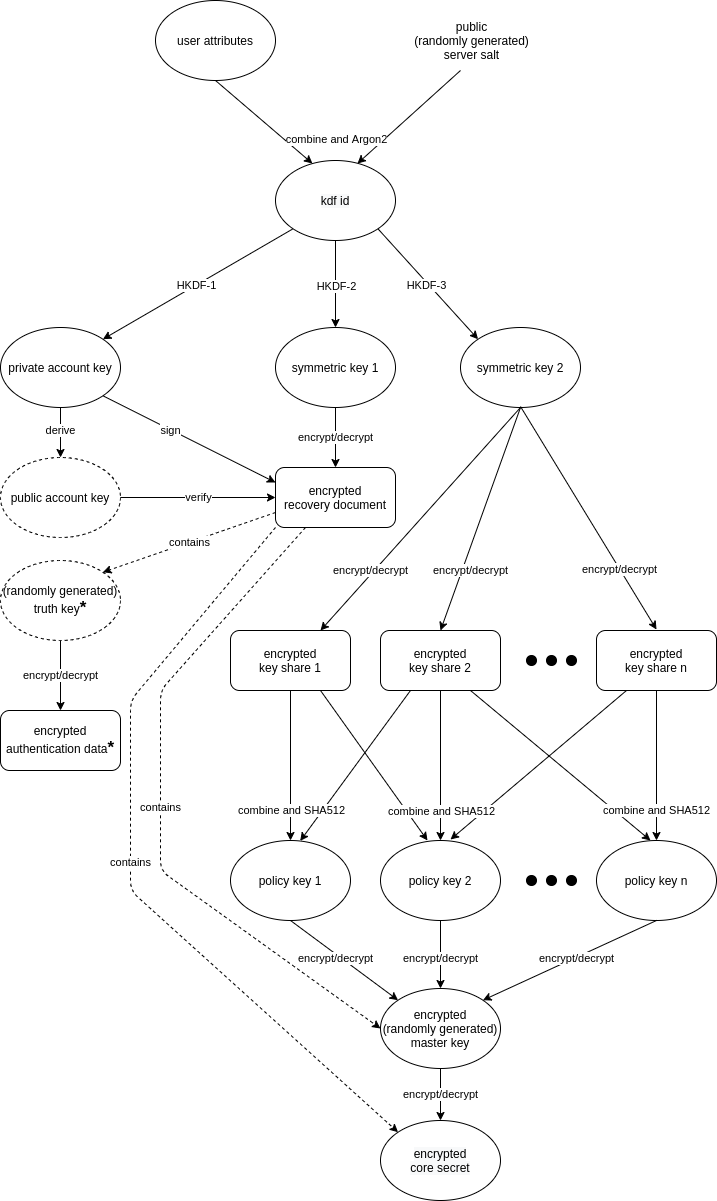
\includegraphics[scale=0.48]{images/keys_anastasis.png}
	\caption{Secrets used in Anastasis}
	\label{fig:keys_anastasis}
\end{figure}

\noindent In the following the keys shown in the Figure~\ref{fig:keys_anastasis} on
page~\pageref{fig:keys_anastasis} are explained:

\begin{description}
	\item[kdf id] {The {\em kdf id} is derived from the user attributes and a
	randomly generated public and constant salt value provided by the escrow provider using Argon2. It is used to derive
	the {\em private account key}, the {\em symmetric key 1} and the {\em symmetric key 2}.}
	\item[private account key] {The {\em private account key} is used to sign the {\em encrypted
	recovery document}. It is derived from the {\em identity key} using {\em HKDF-1}}.
	\item[public account key] {The {\em public account key} is derived from its corresponding
	{\em private account key}. It used to verify the signature of the {\em encrypted recovery
	document} and also is the identifier of the user which is needed by the provider.}
	\item[symmetric key 1] {The {\em symmetric key 1} is derived from the {\em identity key} using
	{\em HKDF-2}. It is used to encrypt and decrypt the {\em encrypted recovery document} which is stored by
	the provider.}
	\item[symmetric key 2] {The {\em symmetric key 2} is derived from the {\em identity key} using
	{\em HKDF-3}. It is used to encrypt and decrypt the different {\em encrypted key shares} which
	are stored by the escrow providers.}
	\item[truth key] {The {\em truth key} is randomly generated for each {\em encrypted authentication data}
	  and is stored within the {\em encrypted recovery document}. It may later be disclosed by the user to
          the escrow provider to let it decrypt the {\em encrypted authentication data} which allows the provider
          to then run the recovery authorization process.}
	\item[master key] {The {\em master key} is randomly generated and is used to encrypt and decrypt the
	{\em encrypted core secret} which is stored within an {\em encrypted recovery document}. The {\em encrypted master key} also is stored within the {\em encrypted recovery document}.}
	\item[policy key] {The {\em policy keys} are used for encryption and decryption of the {\em encrypted master key}. A {\em policy key} is constructed by hashing a specific combination of {\em key shares} specified by the
	user. For hashing SHA512 is used here.}
\end{description}
\newpage

\begin{figure}[H]
	\centering
	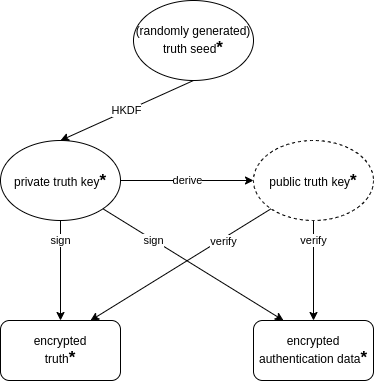
\includegraphics[scale=0.48]{images/truth_anastasis.png}
	\caption{Key generation for signing of encrypted ``Truth'' data in Anastasis}
	\label{fig:truth_keys}
\end{figure}

\noindent In the following the keys shown in the Figure~\ref{fig:truth_keys} on
page~\pageref{fig:truth_keys} are explained:
\begin{description}
\item[truth seed] {Clients generate a random {\em truth seed} for each truth
  which is stored in the encrypted recovery document.}
\item[private truth key] {{\em Private keys} are derived per truth upload. They
  are used to sign the uploaded data. This way, the escrow provider
  can later prove that they preserved the data correctly. We use EdDSA~\cite{josefsson2017} for
  the signatures.}
\item[public truth key] {{\em Public keys} are used to identify the truth
  in the provider's database. Providers only store the first truth upload with
  a valid signature. Changes to truth are thus not possible, clients must
  create a fresh seed for every upload.}
 \end{description}



\subsection{Adversary model}

The adversary model of Anastasis has two types of adversaries: {\em
  weak adversaries} which do not know the user’s identifier (the {\em
  kdf id}), and {\em strong adversaries} which somehow do know a
user’s identifier. Against weak adversaries, the system guarantees
full confidentiality, except for a provider-specific public account
key which links certain requests from the same user, and the data necessary
for authentication. The latter is only disclosed to the providers when
the user requests key recovery. Weak adversaries cannot break
confidentiality even if all escrow providers are part of a conspiracy
of weak adversaries.  For strong adversaries, breaking confidentiality
of the core secret still requires that a sufficient subset of the
Anastasis escrow providers must have colluded with the strong
adversary. The user can specify a set of policies which determine
which Anastasis escrow providers would need to collude to break
confidentiality. These policies also set the bar for the user to
recover their core secret.

Anastasis providers are also not individually trusted to provide
availability or authenticity. Users can specify multiple policies, and
satisfying any one of the policies would allow them to recover their
core secret assuming the subset of providers specified in the policy
is available (and preserved the authenticity of the data).  As clients
sign their uploads, they can verify the authenticity of the data
returned by checking the signatures.  Only strong adversaries are able
to forge signatures, so they could create fraudulent recovery
documents and/or key shares resulting in invalid restored core
secrets. However, because uploads are never destructive, strong
adversaries can only succeed in breaking availability if they collude
with a subset of escrow providers that are present in all policies
selected by the user.

Thus, users can improve confidentiality by having many different
escrow providers in their policies, and improve availability by having
many policies with few escrow providers. Anastasis does not resolve
this trade-off, but allows users to make individual choices and gives
them agility with respect to the parties whom they offer their
trust, resulting in trust agility~\cite{marlinspike2011}.


\subsection{Encryption of the core secret}

The {\em core secret} of the user is (AES)~\cite{heron2009} encrypted using a symmetric
{\em master key}.  Recovering the master key requires the user to
satisfy a {\em policy}. Policies specify a set of escrow methods, each
of which leads the user to a {\em key share}. Combining those key
shares (by hashing) allows the user to obtain a policy key, which can
be used to decrypt the master key.  There can be many policies,
satisfying any of these will allow the user to recover the master key.

Which escrow methods are combined into which policies and which
providers are involved can be different for each user. As users are
unlikely to remember all the details, Anastasis needs a way to
remember the specific configuration a user made.

This process description is provided in a {\em recovery document}.

% Figure~\ref{fig:recoverydoc} gives an example for a the contents of
% a recovery document.
% FIXME: actually include example!


\subsection{The recovery document}

A {\em recovery document} includes all the information a user needs to
recover access to their core secret. It primarily identifies a set of
{\em encrypted key shares} which have been entrusted to different
Anastasis providers. For each key share, the recovery document
specifies the respective Anastasis provider and also prescribes the
{\em authentication method}, which specifies how the user should
convince the Anastasis server that they are authorized to retrieve the
encrypted key share.  Authentication methods can for example include
SMS-based verification, video-identification or a security question.

For each authentication method, specific Anastasis providers are separately
provided (see Section~\ref{sec:truth}) with the associated {\em encrypted key
  share} and (separately encrypted) {\em authentication
  data}. Anastasis operators may learn the authentication data during
the recovery process to authenticate the user. Examples for
authentication data would be a phone number (for SMS), a picture of
the user (for video identification), or the (hash of) a security
answer. A strong adversary is assumed to be able to learn the
authentication data, while weak adversaries must not (except if they
are the provider and then they may learn it only during key recovery).

The recovery document also specifies {\em policies}, which describe
the combination(s) of the key shares (and thus authentication
processes) that would suffice to obtain access to the core secret. For
example, a policy could say that the authentication methods ``$A$ and
$B$'' suffice, and a second policy may permit ``$A$ and $C$''. A
different user may choose to use the policy that ``$A$ and $B$ and
$C$'' are all required. Anastasis imposes no limit on the number of
policies in a recovery document, or the set of providers or
authentication methods involved in guarding a user’s secret.

Weak adversaries must not be able to deduce information about a user’s
recovery document (except for meta data such as its length or
approximate creation time, which may be exposed to an adversary which
monitors the user’s network traffic or operates an escrow provider).


\subsection{Identity-derived encryption}

To start, a user provides their private (alas not really secret),
unique and unforgettable user attributes as a seed to identify their
account. For example, this could be a social security number together
with their full name. Specifics may depend on the cultural context, in
this document we will simply refer to this information as the
{\em user attributes}.

For each Anastasis provider, a {\em kdf id} key is derived from the
user’s attributes and a provider salt using Argon2~\cite{BDK2016}, a
computationally expensive cryptographic hash function. Using an
expensive hash algorithm is assumed to make it harder for a weak
adversary to determine user attributes by brute force guessing.  The
salt ensures that the keys for the same user cannot be easily
correlated across the various Anastasis servers.  However, it is
assumed that a strong adversary performing a targeted attack can
compute the {\em kdf id}s.

The listing in Figure~\ref{fig:argon2} provides pseudo-code for
the computation of the {\em kdf id}. The inputs are:

\begin{description}
	\item[attributes] {The personal attributes provided by the user.}
	\item[server\_salt]{The salt from the Anastasis provider.}
	\item[keysize]{The desired output size of the KDF, here 32 bytes.}
\end{description}

\begin{figure}[H]
\begin{lstlisting}
user_identifier_derive(attributes, server_salt, keysize)
{
  kdf_id = Argon2(attributes, server_salt, keysize)
  return kdf_id
}
\end{lstlisting}
\caption[Use of Argon2 to derive user attributes]{The user's attributes are hashed with Argon2, to provide a
  kdf\_id which will be used to derive other keys later. The hash must
  also be made over the respective provider's server\_salt. This
  ensures that the kdf\_id is different on each server. The use of
  Argon2 and the respective server\_salt are intended to make it
  difficult to brute-force kdf\_id values and help protect user’s
  privacy. Also this ensures that the kdf\_ids on every server
  differs. However, we do not assume that the identifier or the
  kdf\_id cannot be determined by an adversary performing a targeted
  attack, as a user’s identifier is likely to always be known to state
  actors and may likely also be available to other actors.}
\label{fig:argon2}
\end{figure}

Anastasis derives symmetric key material --- but not the master secret --- from the {\em kdf id} using different HKDFs~\cite{krawczyk2010}.

When confidential data --- such as the recovery document or the truth
--- is uploaded to an Anastasis server, the respective payload is
encrypted using AES-GCM with the respective symmetric key and
initialization vector derived key material as shown in
Figure~\ref{fig:keys_anastasis} and a high-entropy nonce.  The nonce
and the GCM tag are prepended to the ciphertext before being uploaded
to the Anastasis server. This is done whenever confidential data is
stored with the server, so both for encrypted authentication data
(\texttt{/truth} uploads) and encrypted recovery documents
(\texttt{/policy} uploads).

To ensure that the key derivation for the encryption of the recovery
document differs fundamentally from that of an individual key share,
we use different salts for different types of operations (“erd” and
“eks” respectively):

\begin{lstlisting}
encryption_key_create(kdf_id, salt, nonce)
{
iv, key = HKDF (kdf_id, nonce, salt, keysize + ivsize)
return iv,key
}
\end{lstlisting}

\begin{description}
	\item[HKDF()] {The HKDF-function uses to phases: First we use HMAC-SHA512 for the extraction phase, then HMAC-SHA256 is used for expansion phase.}
	\item[kdf\_id] {Hashed identifier.}
	\item[keysize] {Size of the AES symmetric key, here 32 bytes.}
	\item[ivsize] {Size of the AES GCM IV, here 12 bytes.}
	\item[nonce] {32-byte nonce, must never match “ver” (which it cannot as the length is different). Of course, we must avoid key reuse. So, we must use different nonces to get different keys and ivs (see below).}
	\item[key] {Symmetric key which is later used to encrypt the documents with AES256-GCM.}
	\item[iv] {IV which will be used for AES-GCM.}
\end{description}


\begin{lstlisting}
encrypt(kdf_id, data, salt)
{
nonce = generate_random_bytes(32)
iv, key = encryption_key_create(kdf_id, salt, nonce)
encrypted_data, aes_gcm_tag =  AES256_GCM(data, iv, key)
encrypted_data = nonce + aes_gcm_tag + encrypted_data
return encrypted_data
}

key_share_encrypt(kdf_id, key_share)
{
encrypted_key_share = encrypt(kdf_id, key_share, "eks")
return encrypted_key_share
}

recovery_document_encrypt(kdf_id, recovery_document)
{
encrypted_recovery_document =
encrypt(kdf_id, recovery_document, "erd")
return encrypted_recovery_document
}

\end{lstlisting}

\begin{description}
	\item[encrypted\_recovery\_document] {The encrypted recovery document which contains the authentication methods, policies and the encrypted core secret.}
	\item[encrypted\_key\_share] {The encrypted key\_share which the escrow provider must release upon successful authentication.}
	\item[nonce] {Nonce which is used to generate keys and ivs which are used for the encryption. The nonce must contain either eks or erd.}
	\item[encrypted\_data] {The encrypted data contains the either a recovery document or a key share which was encrypted and the nonce and the aes\_gcm\_tag. To be able to decrypt it the first 32 Bytes are the nonce and the next 12 Bytes are the aes\_gcm\_tag.}
\end{description}


\subsection{Authenticity of recovery documents}

\texttt{/policy/} requests are used to upload new encrypted recovery
documents. For users to authorize \texttt{/policy} operations, we need
an account key pair.  Thus, in addition to the symmetric keys, an
EdDSA-based {\em account key} is derived from the {\em kdf id} (see
Figure~\ref{fig:keys_anastasis}) and used to identify the ``account''
of the user at each Anastasis server.  EdDSA public keys are always
points on Curve25519 and represented using the standard 256-bit
Ed25519 compact format. The binary representation is converted to
Crockford Base32 when transmitted inside JSON or as part of URLs in
the RESTful API of Anastasis (see Section~\ref{sec:serverarch}).
EdDSA signatures are also provided in Crockford Base32-encoding and
transmitted using the HTTP header
\texttt{Anastasis-Account-Signature}.  Encrypted recovery documents
are stored using the public account key as the identifier.

As the account keys are derived from the {\em kdf id} --- which strong
adversaries are assumed to know ---, we cannot assure that the corresponding
private account key is truly secret. Thus, policy operations must
never be destructive: A strong adversary can derive the private key
and access (and with the {\em kdf id} also decrypt) the user’s
recovery document (but not the core secret!), and also upload a new
version of the encrypted recovery document. However, because uploads
are not destructive, even a strong adversary cannot delete an existing
version and thus cannot break availability.

For the generation of the private key we use the {\em kdf id} as the
entropy source, hash it to derive a base secret which will then be
processed to fit the requirements for EdDSA private keys. From the
private key we can then generate the corresponding public key. Here,
the string “ver” is used for the salt value for the HKDF to ensure
that the result differs from other cases where we hash {\em kdf id}:

\begin{lstlisting}
eddsa_keys_create (kdf_id, salt, keysize)
{
  ver_secret = HKDF(kdf_id, salt, keysize)
  eddsa_priv = ver_secret
  eddsa_pub = get_eddsa_pub(eddsa_priv)
  return eddsa_priv, eddsa_pub
}
\end{lstlisting}

\begin{description}
	\item[HKDF()] {The HKDF-function uses to phases: First we use HMAC-SHA512 for the extraction phase, then HMAC-SHA256 is used for expansion phase.}
	\item[kdf\_id] {Hashed identifier.}
	\item[salt] {Is used that different keys are generated, the salt here is "ver".}
	\item[key\_size] {Size of the output, here 32 bytes.}
	\item[ver\_secret] {Derived key from the kdf\_id, serves as intermediate step for the generation of the private key.}
\end{description}

\begin{description}
	\item[eddsa\_priv] {The generated EdDSA private key.}
	\item[eddsa\_pub] {The generated EdDSA public key.}
\end{description}


\subsection{Account signatures}

The EdDSA account keys are used to sign the encrypted recovery
document sent from the client to the server.

% FIXME: "everything"? I don't think we can sign the encrypted truth
% with the eddsa_priv, as that would link the truth to the ERD.
% We need ANOTHER account key here, one per truth + provider?

\begin{lstlisting}
(anastasis-account-signature) = eddsa_sign(h_body, eddsa_priv)
ver_res =
  eddsa_verifiy(h_body, anastasis-account-signature, eddsa_pub)
\end{lstlisting}

\begin{description}
	\item[anastasis-account-signature] {Signature over the SHA-512 hash of the body using the purpose code TALER\_SIGNATURE\_ANASTASIS\_POLICY\_UPLOAD (1400) (see GNUnet EdDSA signature API for the use of purpose).}
	\item[h\_body] {The hashed body.}
	\item[ver\_res] {A Boolean value. True: Signature verification passed, False: Signature verification failed.}
\end{description}

\noindent
When requesting \texttt{/policy} downloads, the client must also provide a signature:
\begin{lstlisting}
(anastasis-account-signature) = eddsa_sign(version, eddsa_priv)
ver_res =
  eddsa_verifiy(version, anastasis-account-signature, eddsa_pub)
\end{lstlisting}

\begin{description}
	\item[anastasis-account-signature] {Signature over the SHA-512 hash of the body using the purpose code TALER\_SIGNATURE\_ANASTASIS\_POLICY\_DOWNLOAD  \\
	(1401) (see GNUnet EdDSA signature API for the use of purpose).}
	\item[version] {The version requested as a 64-bit integer, for the “latest version”.}
	\item[ver\_res] {A Boolean value. True: Signature verification passed, False: Signature verification failed.}
\end{description}


\subsection{Authenticity of truth} \label{sec:truth}

\texttt{/truth/} requests are used to upload encrypted authentication data
and encrypted key shares to an Anastasis escrow service.  As an additional
layer of protection, an Anastasis escrow service cannot link truth data to
policy data, except maybe by observing the timing of the requests.

Anastasis uses EdDSA-based {\em truth key}s to identify truth
objects. For those, the truth keys are derived from a {\em truth
  seed}, as show in Figure~\ref{fig:truth_keys}.  The private truth
key is used to authorize the truth upload. The signatures also
authenticate the encrypted key shares returned from the Anastasis
provider during recovery.  The signature process for truth is
analogous to that for accounts.


\subsection{Availability considerations}

Anastasis considers two main threats against availability. First, the
Anastasis server operators must be protected against denial-of-service
attacks where an adversary attempts to exhaust operator’s
resources. The API protects against these attacks by allowing
operators to set fees for expensive operations. Furthermore, all data stored
comes with an expiration logic, so an attacker cannot force servers to
store data indefinitely.

A second availability issue arises from strong adversaries that may be
able to compute the account keys of some user. While we assume that
such an adversary cannot successfully authenticate against the truth,
the account key does inherently enable these adversaries to upload a
new policy for the account. This cannot be prevented, as the
legitimate user must be able to set or change a policy using only the
account key. To ensure that an adversary cannot exploit this, policy
uploads first of all never delete existing policies, but merely create
another version. This way, even if an adversary uploads a malicious
policy, a user can still retrieve an older version of the policy to
recover access to their data. This append-only storage for policies
still leaves a strong adversary with the option of uploading many
policies to exhaust the Anastasis server’s capacity. We limit this
attack by requiring a policy upload to include a reference to a
payment identifier from a payment made by the user. Thus, a policy
upload requires both knowledge of the identity and making a
payment. This effectively prevents and adversary from using the
append-only policy storage from exhausting Anastasis server capacity.


\section{Implementation}

The Anastasis is written in C. We decided to use C because of the
various dependencies, including cryptographic libraries.  Especially,
GNU Taler and Sync, which are working in concert with Anastasis, are
also written in C. Using the same language makes integration and
testing of Anastasis much easier.

The whole Anastasis application consists of multiple components.
Figure~\ref{fig:secret_split:overview} gives an overview over all the
components.

\begin{figure}[H]
	\centering
		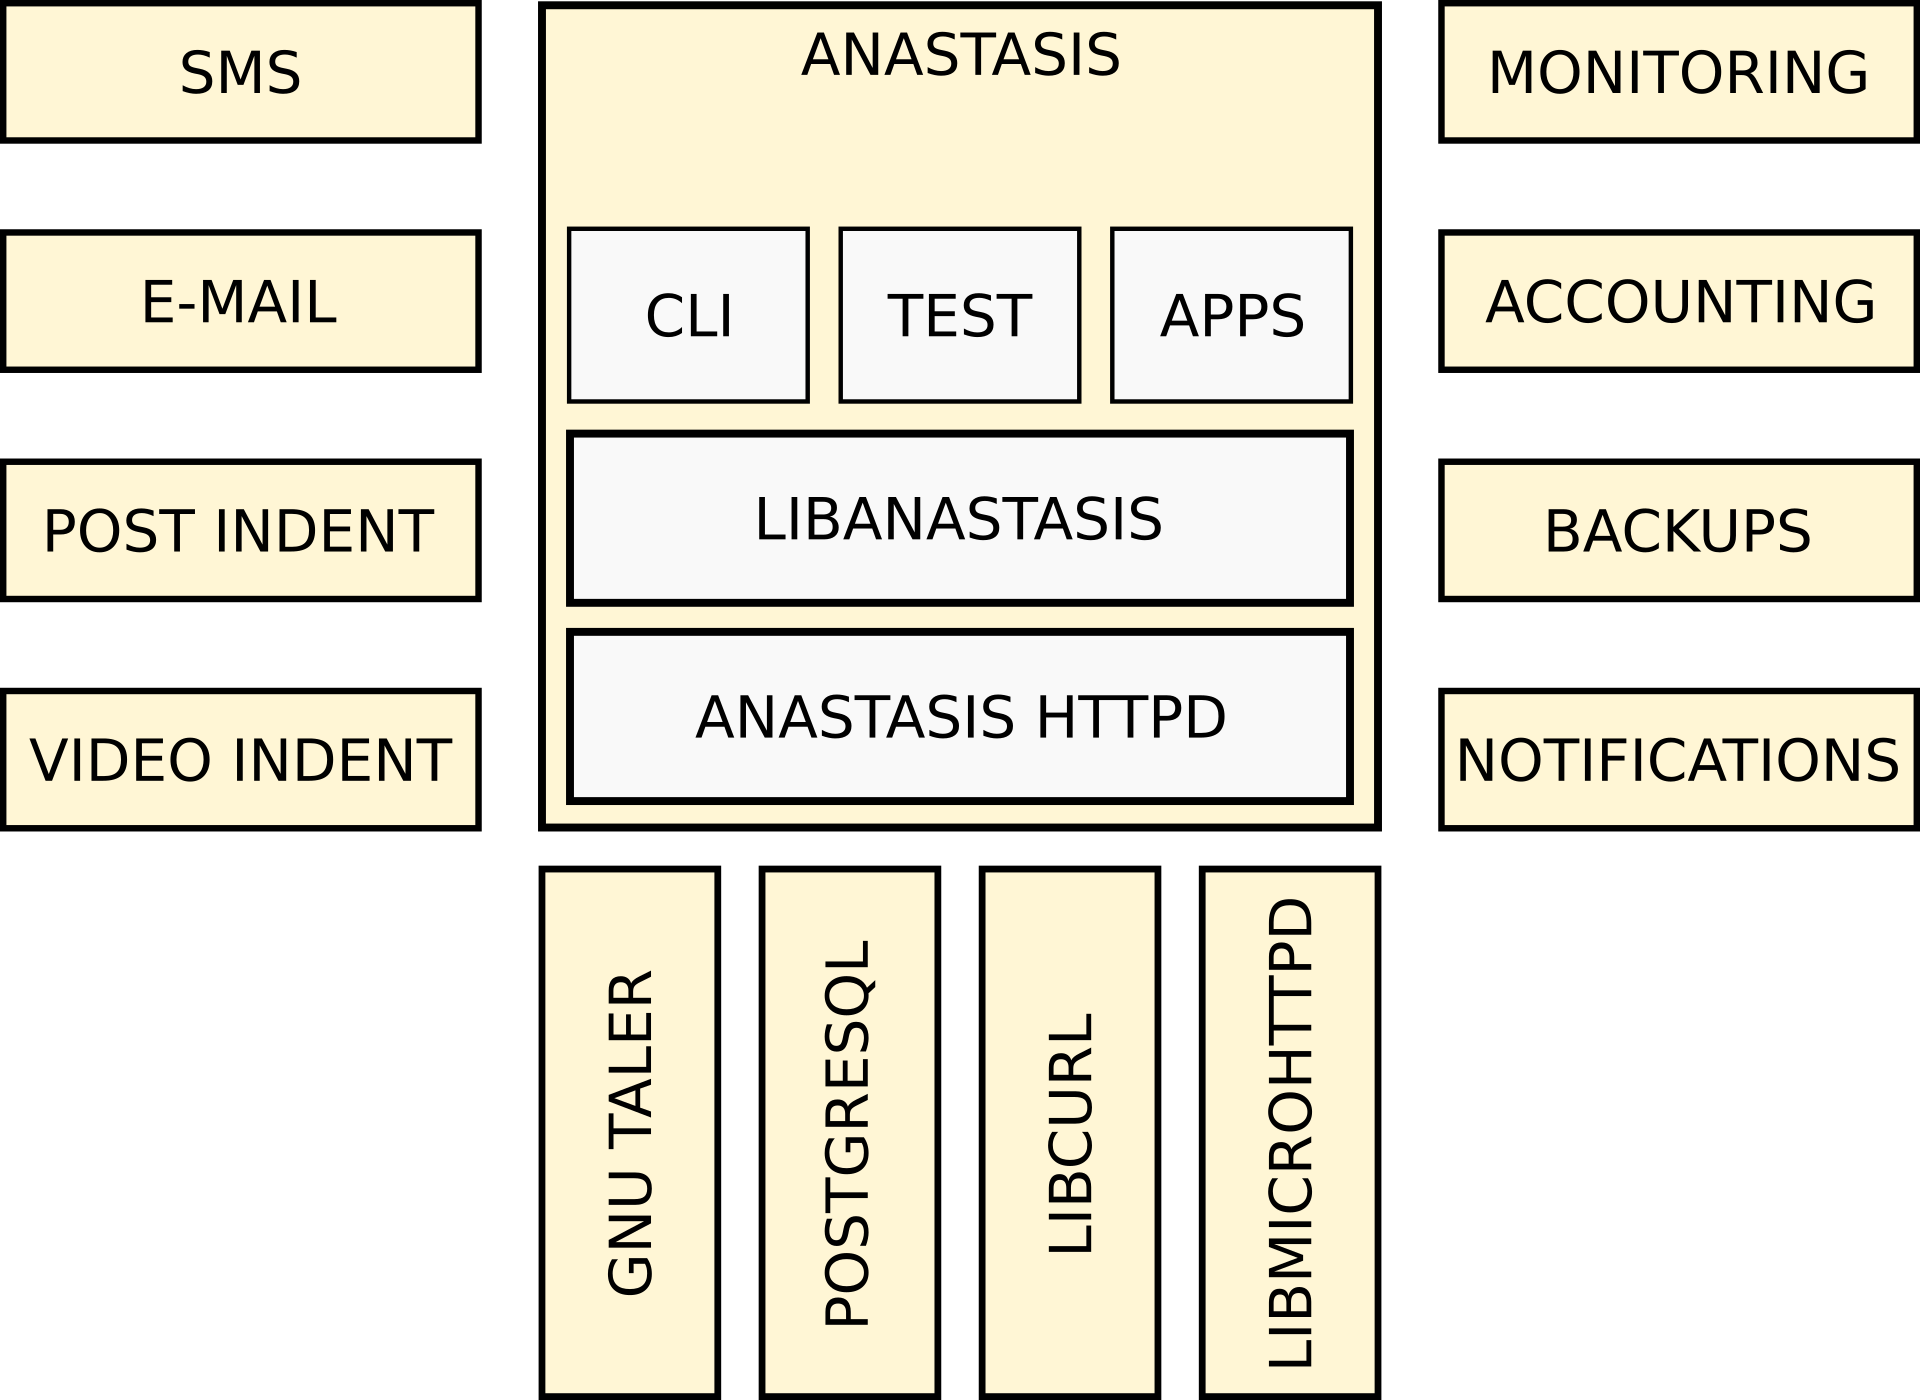
\includegraphics[scale=0.5]{images/system-architecture.png}
	\caption{System architecture overview}
	\label{fig:system_arch:overview}
\end{figure}

\noindent In the center is the core implementation of Anastasis.
On the left are some of the planned authentication methods from the
application. On the right side of the box are the core parts which are
necessary to operate Anastasis commercially. These parts are
anticipated for a production deployment, but not part of the
implementation for this thesis.

At the bottom section are the external libraries used for the project.
These libraries are presented in Section~\ref{sec:libraries}.
\newpage


\subsection{System architecture}

This graphic shows the basic architecture of the Anastasis
application. It shows a simplified flow of the application. The
details of each component are explained later.

\begin{figure}[H]
	\centering
		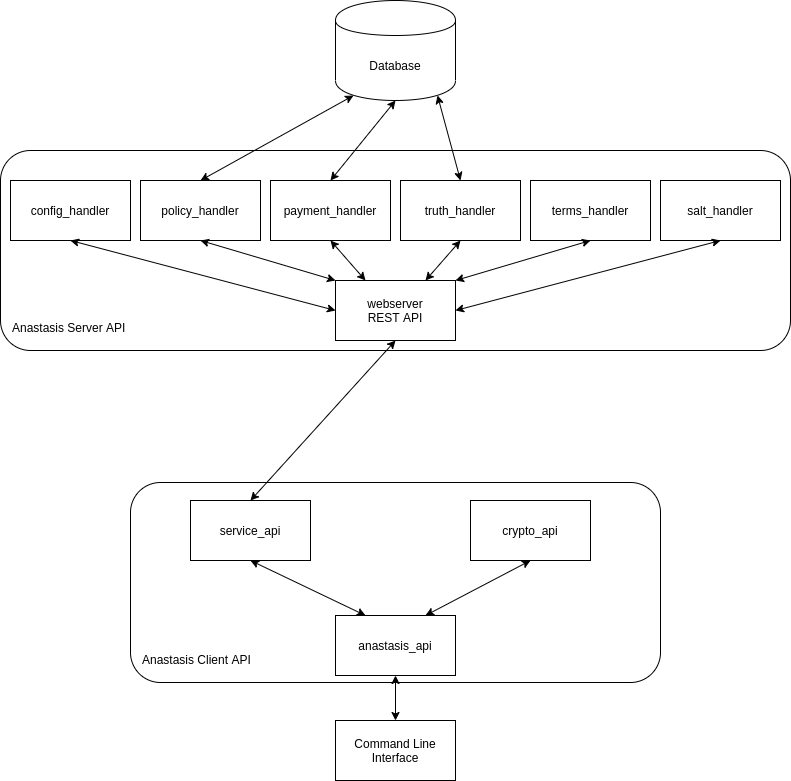
\includegraphics[scale=0.4]{images/system_design.png}
	\caption{System design overview}
	\label{fig:system_design}
\end{figure}

\begin{enumerate}
\item The Anastasis CLI interacts with the Anastasis API. The
  Anastasis API is responsible for triggering interactions with the
  user, and also manages the interactions between the
  various client-side components.
\item After the user provided their unforgettable secret, the
  Crypto API derives the needed key material for the further
  communication. This is simplified, in reality the client would first
  need to download the server salt to generate the user keys.  The
  crypto API is later also responsible for the decryption and
  encryption of the data, sent or received from the server.
\item The Service API is responsible for the communication with the
  Anastasis server. The Anastasis API sends the previously generated
  data and the user selected request to the service.
  The Service API is also responsible to handle
  the server's response to the request.
\item The central webserver logic handles HTTP requests sent to it by the
  clients. It will dispatch requests to the corresponding handler. The
  webserver's core logic also returns the response and the status code
  of the operation to the client application.
\item Each REST endpoint of the Anastasis server is implemented by
  a specific handler. The handler processes the requests, typically
  by storing or looking up the requested
  data with the database. When the request is finished, the handler will
  send back the data or the status code to the webserver's core logic.
\end{enumerate}


\subsection{Server architecture} \label{sec:serverarch}

The Anastasis server architecture consists of two components. A web
server with a REST API and a PostgreSQL database. The structure of
these two components is shown in Figure~\ref{fig:anastasis:server}.

\begin{figure}[H]
	\centering
	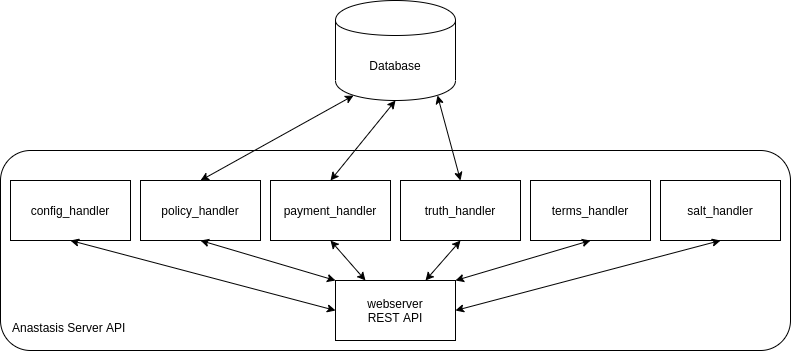
\includegraphics[scale=0.45]{images/server_api.png}
	\caption{Anastasis server architecture}
	\label{fig:anastasis:server}
\end{figure}

The webserver of Anastasis provides a RESTful API. For a detailed
documentation of the REST API, see
appendix ~\ref{appendix_server_api}.

\newpage
\subsubsection{Database}

The database schema of Anastasis is shown in
Figure~\ref{fig:anastasis_database}.
\begin{figure}[H]
	\centering
	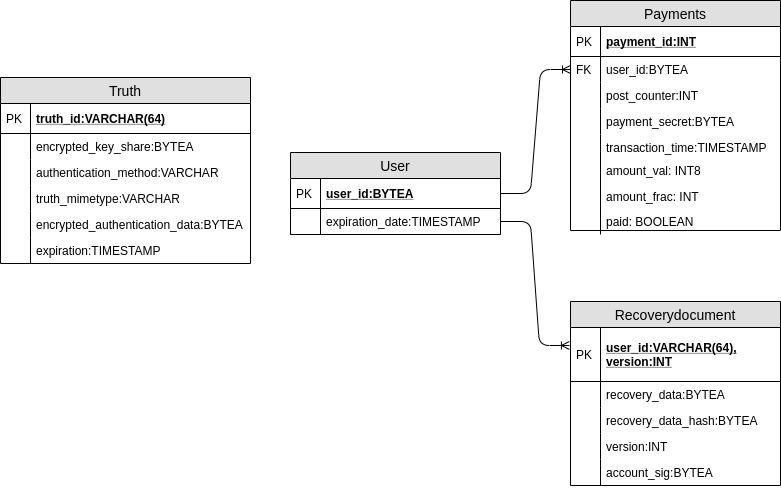
\includegraphics[scale=0.5]{images/anastasis-db.png}
	\caption{Anastasis database schema}
	\label{fig:anastasis_database}
\end{figure}

The database schema consists of four main tables:

\begin{itemize}
\item The {\em Truth} table is responsible for storing the key shares and
  its authentication method. The key share and the authentication data are stored
  encrypted in the database. The authentication data is only decrypted during
  authentication. The key share is never decrypted for the
  server. This protects the privacy of the customer. Likewise, the
  user data is protected after a possible theft.
\item The {\em User} table contains the identification of the user and an
  expiration timestamp. This timestamp is a subscription period. This
  timestamp is updated after each payment the user makes. Users for
  whom the subscription has expired are periodically deleted.
\item The {\em Payments} table contains the details of a payment from a
  user. The payment is used either for the post-counter or the
  subscription. The post-counter is decremented after each upload of a
  recovery document. The user can only upload the recovery document if
  the provided payment contains a post-counter which is at least 1.
  Through this measure we can prevent people from maliciously filling
  our database.
\item The {\em Recoverydocument} table contains the recovery
  information. The recovery document is stored encrypted in the
  database. This offers better protection, as explained earlier for
  the Truth table. Each recovery document record also contains a
  version, a hash of the recovery document and a signature. The
  version attribute allows the user to lookup a specific version of
  the document. The hash is used to check if the user uploads a
  duplicate of the document. The signature attests the
  integrity of the recovery data.
\end{itemize}


\subsubsection{Authentication methods}

This section describes an overview over the different possible
authentication methods for Anastasis. In our implementation only the
secure question is implemented. The other methods are just explained
how they would be implemented.

In all cases, the authentication process begins by the user decrypting
their (encrypted) recovery document, which contains a list of Anastasis
providers, associated authentication methods, truth\_seeds and associated
truth encryption keys.  The recovery process than varies slightly
depending on the authentication method.

\paragraph{SMS (sms)}

The user tells the server with a request that they wants to authorize
key recovery (via GET /truth/\$TRUTH\_PUB), providing a way to decrypt the
truth with the phone number. The server will then generate a \$PIN and
send it via an SMS provider to the stored number in the truth
object. The client then must send another request with the sent \$PIN
(via GET /truth/\$TRUTH\_PUB?response=\$PIN). The server can now check
if the two PINs match. Upon success, the server returns the encrypted
key share.

\paragraph{Video identification (vid)}

This method allows the user to identify via video-call.  Since the
respective images must be passed on to the video identification
service in the event of password recovery, it must be ensured that no
further information about the user can be derived from them.  Hence,
the user's client software must try to delete metadata that could
result in accidental information leakage about the user from the image
before encrypting and uploading it to the Anastasis provider.

For recovery, the user must first send a request to server that they
wants to authorize recovery (GET /truth/\$TRUTH\_PUB).  The Anastasis
provider will then decrypt the user's image and send a request with a
\$TOKEN to a video authentication provider that a user wants to
authenticate, and respond to the user with a link to a video
conference.  The video authentication provider then checks via video
conference that the user in the image is the same that they have on
the video link. Upon success, the video provider releases the \$TOKEN
to the user.  The client then must send another request with the
\$TOKEN (via GET /truth/\$TRUTH\_PUB?response=\$TOKEN). The Anastasis
provider checks that the tokens match, and upon success returns the
encrypted key share.

\paragraph{Post identification (post)}

The user tells the Anastasis provider with a request that they want
to authenticate using Post identification (GET /truth/\$TRUTH\_PUB).  The
Anastasis provider uses the request to decrypt the user's truth to
determine the user's postal address, and sends them letter containing
a \$PIN.  Upon receiving the letter, the client then has to send
another request with the \$PIN (GET /truth/\$TRUTH\_PUB?response=\$PIN). The
server can now check if the two PINs match. Upon success the server
will release the encrypted key share.

\paragraph{Security question (qa)}

The user provided Anastasis with a secure question and a (normalized)
answer.  The secure question becomes part of the encrypted recovery
document, and is never disclosed to weak adversaries, even during
recovery.  The encrypted truth on the server only contains a (salted)
hash of the answer. The Anastasis provider cannot learn the plaintext
answer. Because of the salt, and it cannot mount a confirmation attack
either.

If the user wants to recover the key share from the server, they must
provide the (salted) hash of the answer to the security question (via
GET /truth/\$TRUTH\_PUB?response=\$HASH). The server then checks if the
stored and the provided hash match. Upon success the server responds
with the encrypted key share.


\subsection{Client architecture}

The Anastasis client architecture consists of two main components. A client
API which communicates with the server and a command line application
which interacts with the user. The structure of these two components
is shown in Figure~\ref{fig:anastasis:client}.

\begin{figure}[H]
	\centering
	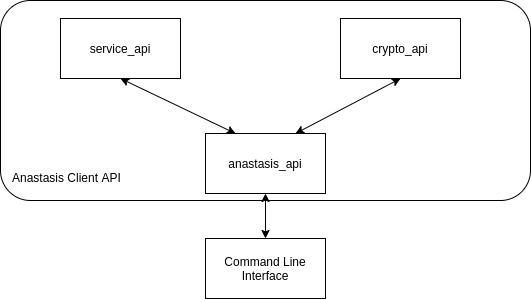
\includegraphics[scale=0.6]{images/client_api.png}
	\caption{Anastasis client architecture}
	\label{fig:anastasis:client}
\end{figure}

The Anastasis client implementation includes three distinctive APIs: a
{\em Crypto API} which provides the different cryptographic functions,
a {\em Service API} which sends the request to the server and the {\em
  Client API} which manages the main data structures and provides an
abstraction for the application.

\subsubsection{Crypto API}

The most important data structures in the crypto API are the following:

\begin{itemize}
  \item
The kdf\_id is a hash code which was generated with Argon2. The
entropy source is the user's unforgettable secret. The kdf\_id is used
to create various key's, for more details see Chapter~\ref{chap:design}.

\begin{lstlisting}
struct kdf_id
{
  Hashcode; //512-bit
}
\end{lstlisting}

\item
The account\_private\_key is used to sign the data and check the signature later. It is a 256-bit EdDSA private key. It is generated with the kdf\_id as entropy source.
\begin{lstlisting}
struct account_private_key
{
  eddsa_private_key;
}
\end{lstlisting}

\item
The account\_public\_key is used as the user identification on the different providers. It is generated from the private\_key.
\begin{lstlisting}
struct account_public_key
{
  eddsa_public_key;
}
\end{lstlisting}

\item
The truth\_key is a randomly generated AES-256 GCM key. It is used to encrypt the user specify data in the truth object.
\begin{lstlisting}
struct truth_key
{
  key; //256-bit
}
\end{lstlisting}

\item
The truth\_seed is a randomly generated nonce with a size of 32 Bytes. It is used to derive a truth\_private\_key
and is stored within an encrypted recovery document.
\begin{lstlisting}
struct truth_seed
{
  nonce; //256-bit
}
\end{lstlisting}

\item
The truth\_private\_key is used to sign the encrypted key share and the encrypted authentication data. It is a 256-bit EdDSA private key. It is generated with the truth seed as entropy source.
\begin{lstlisting}
struct truth_private_key
{
   eddsa_private_key;
}
\end{lstlisting}

The truth\_public\_key is used as the user identification on the different providers in case of uploaded truths. It is generated from the truth private key.
 \begin{lstlisting}
struct truth_public_key
{
  eddsa_public_key;
}
\end{lstlisting}


\item
Anastasis needs different symmetric keys to encrypt data for example, the recovery document. These symmetric keys are all 256-bit large hashcodes. These symmetric keys are generated through the key routine defined in Implementation Key usage.
\begin{lstlisting}
struct symmetric_key
{
  hashcode; //256-bit
}
\end{lstlisting}

\item
Each policy has a separate policy\_key. The key is used to encrypt the master\_key.
The policy\_key is also a AES-256 GCM key. It is generated through the combination of a set of key\_shares.
\begin{lstlisting}
struct policy_key
{
  hashcode; //256-bit
}
\end{lstlisting}

\item
Every truth object contains a key\_share. A key\_share is a 256-bit random generated bit sequence.
\begin{lstlisting}
struct key_share
{
  hashcode; //256-bit
}
\end{lstlisting}

\item
Before every encryption a random 256-bit large nonce is generated. This gives the encryption algorithm a random factor.
\begin{lstlisting}
struct nonce
{
  hashcode; //256-bit
}
\end{lstlisting}

\item
To use AES-256 GCM an IV must be generated. It is generated with an HKDF over a salt the kdf\_id and a symmetric key.
\begin{lstlisting}
struct iv
{
  hashcode; //128-bit
}
\end{lstlisting}

\item
The aes\_tag is generated after each encryption, it is later used to check the integrity of the data.
\begin{lstlisting}
struct aes_tag
{
  hashcode; //128-bit
}
\end{lstlisting}
\end{itemize}

The functions of the crypto API basically provide the canonical set of
cryptographic operations (hash, encrypt, decrypt, etc.)  over these
basic data structures.


\subsubsection{Client API}

The most important data structures in the client API are the following:

\begin{itemize}
  \item
The secret share data structure is used to upload a new recovery document.
\begin{lstlisting}
struct secret_share
{
  kdf_id;
  last_etag;
  policies;
  core_secret;
}
\end{lstlisting}
\begin{itemize}
\item kdf\_id: is used to compute the account public and private key. The hash is 512bit large.
\item last\_etag: this hash is sent with the recovery document. The server will check the hash if the document on the server is the same. This prevents unnecessary uploads. The hash is 512-bit large.
\item policies: is a list of all generated policies the user wants to combine into a recovery document.
\item core\_secret: is the user provided core secret. This is just a binary blob so Anastasis does not have a restriction for the user secret. This could be a for example a private key or a password the user wants to backup.
\end{itemize}

  \item
The recovery information data structure holds a recovery document. It is downloaded within the recovery process and stored inside a recovery data structure.
\begin{lstlisting}
struct recovery_information
{
  struct decryptption_policies;
  struct challenges;
  version;
  salt;
}
\end{lstlisting}
\begin{itemize}
\item decryption\_policies: holds all available policies within the downloaded recovery document.
\item challenges: holds all available authentication methods within the recovery document.
\item version: the version of the downloaded recovery document is stored here.
\item salt: this is the salt used for the generation of the policy keys. The salt is a 512-bit value.
\end{itemize}

\item
The recovery data structure is generated at the start of a secret recovery. It contains all available policies and lists which challenges are solved. Through this
struct the client can check if a policy was solved completely.
\begin{lstlisting}
struct recovery
{
  kdf_id;
  version;
  provider_url;
  salt;
  solved_challenges;
  struct recovery_information;
}
\end{lstlisting}
\begin{itemize}
\item kdf\_id: is used to compute the account public and private key. The hash is 512bit large.
\item version: hold the user desired version he wishes to download. This can be null then the client downloads the latest version.
\item provider\_url: the client will download the recovery document from this provider url.
\item salt: this is the salt of the provider specified in provider\_url.
\item solved\_challenges: this is a list of all solved challenges. This list is updated after each successful authentication. This allows the client to check if a policy is solved.
\item recovery\_information: as previously mentioned this data structure holds the downloaded recover document to process within the recovery
\end{itemize}

\item
A truth data structure is used to upload a new authentication method to a provider. It is identified by the TRUTH\_PUB which the user creates through a HKDF over the truth\_seed. The truth data structure is only used for the secret share process and not for the recovery.
\begin{lstlisting}
struct truth
{
  truth_seed;
  method;
  mime_type;
  encrypted_truth;
  encrypted_key_share;
}
\end{lstlisting}
\begin{itemize}
\item truth\_seed: the truth\_seed is the identification of the truth object.
It is used as entropy source to generate the TRUTH\_PUB, which later identificates the truth object. The truth objects are not linked to the user. A list of these truth\_seeds are stored inside the recovery document, with this the user data is more anonymous.
\item method: this defines which method the user chose to configure, for example SMS, email, secure question.
\item mime\_type: this defines in which format the truth was safed, for example jpeg, png, txt, json.
\item encrypted\_truth: the encrypted truth holds the authentication specific data. It holds for example the hashed answer and the question. It is encrypted with the specific truth\_key which is stored inside the recovery\_document.
\item encrypted\_key\_share: this is the key\_share protected by this truth. It is encrypted with a key which was derived with the kdf\_id of the user. The server will later send this key\_share to the user upon successful authentication.
\end{itemize}
\newpage
\item
The policy data structure is used to create new policies to combine them into the recovery document. The policy data structure is only used for the secret share process.
\begin{lstlisting}
struct policy
{
 truths;
 policy_key;
 salt;
}
\end{lstlisting}
\begin{itemize}
\item truths: every policy has a set of truths which need to be solved to recover the policy\_key
\item policy\_key: the policy\_key is created through the combination of the different key\_shares within each of the truth objects. It is later used to encrypt the master\_key.
\item salt: defines the salt used to create the policy\_key.
\end{itemize}

\item
The decryption\_policy data structure is used in the recovery process. It has slightly different values as the policy structure.
\begin{lstlisting}
struct decryption_policy
{
  truth_seeds;
  encrypted_master_key;
  salt;
}
\end{lstlisting}
\begin{itemize}
\item truth\_seeds: is a list of truth\_seeds which need to be solved to recreate the policy key. Each truth\_seed has a corresponding challenge.
\item encrypted\_master\_key: holds an encrypted version of the master\_key which was used to encrypt the core secret. In every policy lies the same master\_key which was encrypted by the specific policy\_key.
\item salt: defines the salt which was used to create this policy\_key.
\end{itemize}
\newpage
\item
The challenge data structure is used for the several key\_share lookups.
We named the process of authentication on the providers as challenges.
It has slightly different variables as the truth data structure.
\begin{lstlisting}
struct challenge
{
  truth_seed;
  url;
  truth_key;
  method;
  key_share;
  instructions;
}
\end{lstlisting}
\begin{itemize}
\item truth\_seed: Entropy source to generate the TRUTH\_PUB, which identifies the challenge on the server.
\item url: defines the provider URL on which the truth was stored.
\item truth\_key: this key is sent to the server within the authentication procedure. The server can decrypt the truth with this key to start the authentication.
\item method: defines the method of this challenge, for example email, SMS, secure question.
\item key\_share: After each successful authentication the key\_share which was sent by the server will be saved within this variable. It is later used to recreate a policy\_key.
\item instructions: this contains a string with the instructions for the user. This could for example be:” What is your favourite colour?” or” An SMS was sent to the number +41...... please provide the pin”.
\end{itemize}
\end{itemize}

The functions of the client API basically provide a way to
backup a core secret by providing user's identity attributes,
the secret and constructing the policies, as well as a way
to recover a core secred by providing the user's identity
attributes and then satisfying the authentication challenges.


\subsubsection{Service API}

The service API is responsible for sending the requests to the REST
API of the server. The client has implemented functions for every
endpoint.
For more details see REST API documentation in
appendix~\ref{appendix_server_api}.


\newpage
\subsection{Application flow}

This section describes a happy flow of the two protocols of Anastasis,
secret splitting and secret recovery.

\subsubsection{Secret splitting}

Figure~\ref{fig:secret_split} illustrates the secret splitting
process.

\begin{figure}[H]
	\centering
		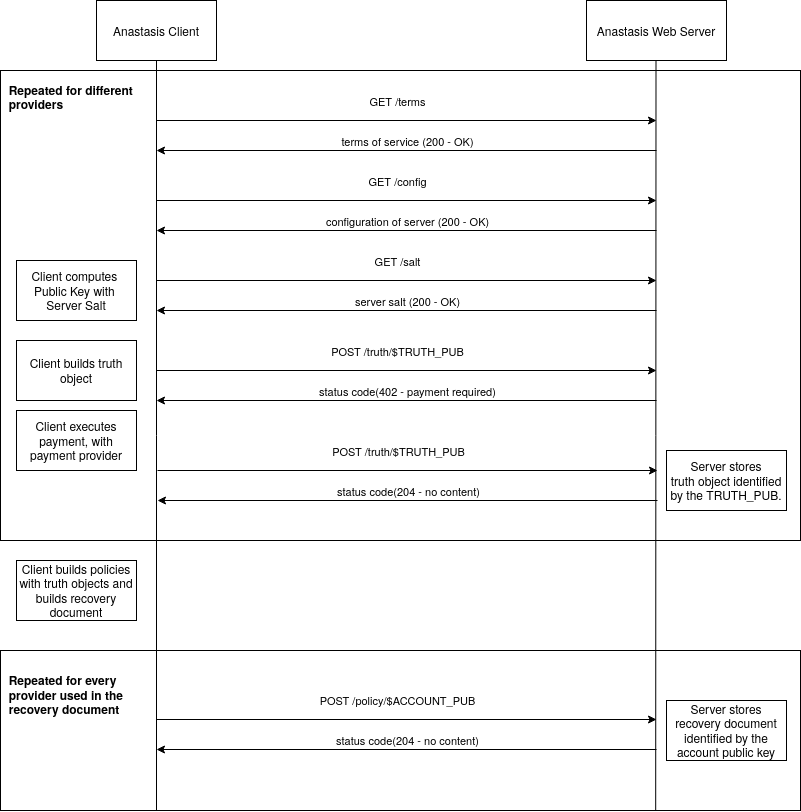
\includegraphics[scale=0.5]{images/secret_split.png}
	\caption{Secret split process}
	\label{fig:secret_split}
\end{figure}
\newpage
\begin{enumerate}
\item The user selects a new escrow provider on which per wants to
  store a truth object.
\item The client software downloads the terms of service for this
  provider (GET /terms). This is also a check if the server is
  available if this command doesn't respond the client will abort the
  process.
\item Next the client requests the server configuration (GET
  /configuration). The configuration lists the available
  authentication methods and the protocol version of the server.
\item The client downloads the server salt (GET /salt). The salt is
  used to generate the server specific account public key, which
  identifies the user.
\item After the user has generated the public key, per will create a
  truth object on the client. The truth object contains all the needed
  information for the recovery for this key share. This truth object
  is sent encrypted to the server and stored under the TRUTH\_PUB the client
  generated (POST /truth/\$TRUTH\_PUB).
\item In this scenario the client has not jet paid for the
  upload. This means the server will respond with the HTTP status code
  \texttt{402 Payment required}. The client first must do a payment with our
  payment provider --- GNU Taler. After the successful payment the client
  will receive a payment identifier. With this payment identifier he
  can resend the previously failed request.
\item The user will now repeat the steps 1-6 until per thinks that they
  have setup a sufficient amount of authentication methods. The user
  can now combine these providers to create policies. For example per
  may have stored three truth objects at three different providers.
  This means per can now define combinations with these providers,
  for example A+B, A+C and B+C. This means the user has three ways to
  recover their secret.
\item After the user has generated the policies the client will
  generate a recovery document. The recovery document contains a list
  of all truth\_seed's used, a list of the policies and the encrypted core
  secret of the user. The client will now send a encrypted recovery
  document to each provider used in the recovery document (POST
  /policy/\$ACCOUNT\_PUB). Through this, the recovery document is
  replicated and recovery can proceed without a single point of
  failure.
\end{enumerate}
\newpage
\subsubsection{Secret recovery}

Figure~\ref{fig:recovery_process} illustrates the recovery process.
\begin{figure}[H]
	\centering
		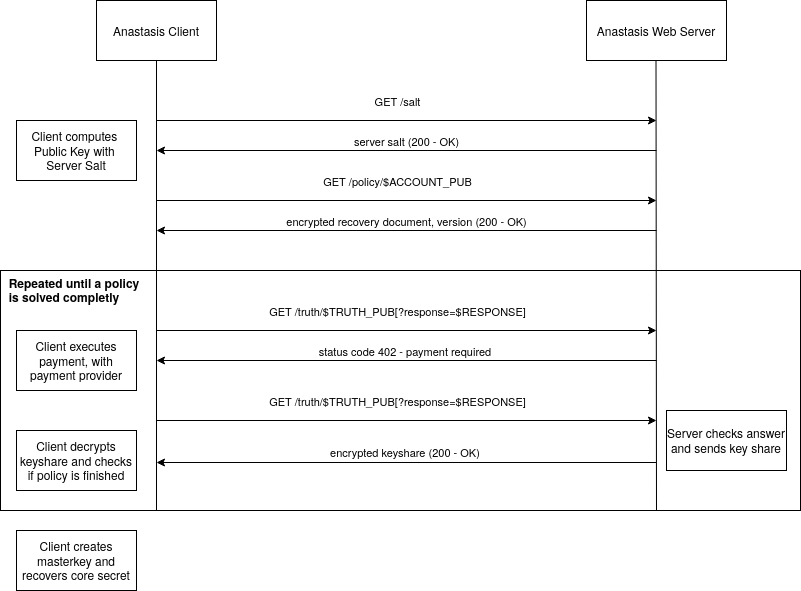
\includegraphics[scale=0.5]{images/recovery_process.png}
	\caption{Secret recovery process}
	\label{fig:recovery_process}
\end{figure}
\begin{enumerate}
\item The user selects a server on which per previously stored a
  recovery document.
\item Next the client downloads the server salt to compute the server
  specific account public key (GET /salt).
\item After the user generated the public key, per will download the
  recovery document. At this point per can define a
  specific version or the latest version of the recovery document. In
  the illustration the client downloads the latest version (GET
  /policy/\$ACCOUNT\_PUB).
\item The client will now decrypt the recovery document and list all
  policies and authentication methods. The user now has to solve these
  challenges. In this example the user has to answer a secure question
  which was sent to them in the recovery document. (GET
  /truth/\$TRUTH\_PUB?response=\$RESPONSE) \\
\item Note the server can define that a challenge has a certain cost,
  in this scenario the server rejects the first request because the
  user has not yet paid for recovery.  After the payment the user can
  resend the request.  After each successfully solved challenge the
  client will check if one of the policies is completely satisfied.
  If all shares needed for one of the policies have been recovered,
  the client will decrypt the core secret and provide it to the user.
\end{enumerate}

Figure~\ref{fig:recovery_process} shows the flow using a secure
question for the authentication challenge. If the user would have
chosen a complex authentication method like SMS or E-Mail, the client
would first need to start the challenge with the request (GET
/truth/\$TRUTH\_PUB). The server would then notify the user that per will
receive some token out of bounds. After that, the user would have to
provide for example the PIN sent to them via SMS with the same request
as before (GET /truth/\$TRUTH\_PUB?response=\$RESPONSE).


\subsection{Client Application Command Line Interface (CLI)}

There are two client applications which interact with the user. First
the Anastasis {\em splitter} and second the Anastasis {\em
  assembler}. The splitter application is responsible for the backup
of the core secret. The assembler is then responsible for the recovery
of the core secret.

Both commands are started with a configuration option ``--me=FILE''
that gives the name of a file with the user's identity attributes.

\subsubsection{Anastasis splitter}

The user starts the assembler by passing a JSON document with their
unforgettable identity attributes (name, social security number, ...).

The following commands are available:

\begin{itemize}
\item server add \$URL: this command lets the user add escrow
  providers. The command will check if a supported escrow service is
  available under the provided URL. Afterwards it will download its
  terms and salt. The server needs to be added before the user can do
  any uploads on it.
\item truth add \$server \$method \$truth: with this command the user
  can upload a truth on a previously added server. The user needs to
  specify the authorization method used and the truth for the
  authorization process, for example the phone number for SMS
  authentication.  The application will check if the server supports the
  provided method before uploading.
\item policy add \$truth1 \$truth2...: after a user has added all the
  truths, per can start to create policies. Per can combine the truths
  in any way they wish. It is also possible to just store one truth in
  a policy, but this is not recommended since it defies the design of
  the application.
\item policy: shows all created policies.
\item truth: shows all created truths.
\item server: shows all added servers.
\item publish \$secret: if the user is finished per can publish the
  configuration. The application will then generate the recovery
  document with the provided information and secret. Afterwards, it
  will upload the recovery document on every server that was used. For
  recovery, the user only needs to remember any one of the servers.
\end{itemize}

Below is an example transcript of an interaction with the splitter:

\begin{lstlisting}
$ anastasis-splitter --me=identity.json
anastasis-splitter> server add $URL1
version: 1.0
annual fee: 4.99 KUDOS,
available policy methods: sms
Server #1 available
anastasis-splitter> server add $URL2
version: 1.0
annual fee: 3.99 KUDOS,
available policy methods: sms, question
Server #2 available
anastasis-splitter> truth add server#1 sms +492452526
Truth #1 added for server #1
anastasis-splitter> truth add server#2 mail "hoehenweg 80, Biel"
Sorry, server #2 does not support 'mail'
anastasis-splitter> truth add question "favorite color" "red"
Truth #2 added
anastasis-splitter> policy add truth#1 truth#2
Policy #1 defined
anastasis-splitter> policy
Policy#1: #truth#1 #truth2
anastasis-splitter> truth
truth#1: server#1 sms  +492452526
truth#2: server#2 question "favorite color" <OMITTED>
anastasis-splitter> truth --secrets
truth#1: sms  +492452526
truth#2: question "favorite color" "red"
anastasis-splitter> server
server#1: http://anastasis.example.com/ methods: sms,
insured up to: 420 KUDOS, cost: 0.4 KUDOS
anastasis-splitter> publish
Server#1 failure: 402 payment required:
payto://pay/ABALSASDFA KUDOS:0.3
Server#2 failure: 402 payment required:
payto://pay/ABALSAADAS KUDOS:0.5
Total: 0.8 KUDOS
# Here: taler-wallet-cli payto://pay/ABALASDFA used to pay!
anastasis-splitter> publish
Server#2 failure: 402 payment required
# Here: taler-wallet-cli payto://pay/ABASDFASDF used to pay!
anastasis-splitter> publish "my super secret"
Thank you for using Anastasis.
$
\end{lstlisting}

\subsubsection{Anastasis assembler}

The user starts the assembler by passing a JSON document with their
unforgettable identity attributes (name, social security number, ...).
They also must pass the URL of an escrow provider which stores their
recovery document, as well as the requested version of the recovery
document. The assembler will then download and decrypt the recovery
document and begin the recovery process.


The following commands are available:
\begin{itemize}
\item truth: shows all available authorization challenges
  from the recovery document and their status (``(-)'' not solved, ``(+)'' solved)
\item policies: shows all available policies in the recovery document and
  the respective status of the truths used in each policy.
\item try \$truth: this command starts an authorization process which
  needs interaction with external services like SMS or email. It shows
  the instructions to follow to authorize release of the share.
\item answer \$truth \$answer: this command tries to answer the
  selected challenge with the provided answer. The application will
  check the answer and give a feedback to the user. Every time a
  challenge is solved, the client API will check if as a result any of
  the policies is completely satisfied.  If any policy was completely
  satisfied, the assembler will print out the recovered core secret
  and exit.
\end{itemize}

Below is an example transcript of an interaction with the assembler:

\begin{lstlisting}
$ anastasis-assembler --import https://anastasis.example.com/
--policy-version=42 --me=identity.json
anastasis-assembler> truth
truth#1(-): KUDOS 0.0 question "favorite color"
truth#2(-): KUDOS 0.4 sms
truth#3(-): KUDOS 2.6 post
anastasis-assembler> policies
policy#1: KUDOS 0.4 truth#1 truth#2 missing
policy#2: KUDOS 3.0 truth#1 truth#2 truth#3 missing
anastasis-assembler> try truth#2
payto://pay/BASDFASD
# SMS arrives asynchronously
anastasis-assembler> answer truth#2 1234
Success truth#2
anastasis-assembler> answer truth#1 "blue"
Failed truth#1
anastasis-assembler> truth
truth#1(-): KUDOS 0.0 question "favorite color"
truth#2(+): KUDOS 0.4 sms
truth#3(-): KUDOS 2.6 post
anastasis-assembler> policies
policy#1: KUDOS 0.0 truth#1 missing
policy#2: KUDOS 2.6 truth#1 truth#3 missing
anastasis-assembler> answer truth#2 "red"
Success truth#2
//One of the policies was solved successfully and the secret is recovered.
Secret was: "my super secret"
$
\end{lstlisting}



\subsection{Libraries} \label{sec:libraries}

In this section the libraries used by Anastasis are presented.

\subsubsection{GNU Taler}

GNU Taler is one of the main reasons why we started to implement
Anastasis, since the application needs a system to back up the private
keys of their users.  ``GNU Taler is a privacy-preserving payment
system. Customers can stay anonymous, but merchants can not hide their
income through payments with GNU Taler. This helps to avoid tax
evasion and money laundering.''~\cite{gnu_taler}

To operate GNU Taler the user needs to install an electronic
wallet. Backups of the wallet are secured with a secret key. Here
comes Anastasis into play, Anastasis will secure this secret key for
the user.

In our implementation GNU Taler is also our payment system. We decided
to use GNU Taler because both Anastasis and GNU Taler are privacy
preserving applications. If we for example used credit cards for
payments the user would no longer be anonymous which is helpful for
the security of Anastasis as it allows us to use the user's name in
the user's identity attributes.  GNU Taler is also a GNU package
and Free Software.~\cite{gnu_taler}
\newpage
\subsubsection{PostgreSQL}

PostgreSQL is a Free/Libre Open Source object-relational
database. PostgreSQL has over 30 years of active development which
makes it a stable and reliable software.

We use PostgreSQL as our database on the Anastasis server. We decided
to use PostgreSQL because it is an open source and lightweight
software which has a big community.  This means there are a lot of
helpful documentations and forums.~\cite{postgresql}

\subsubsection{Libcurl}

Libcurl is a libre URL transfer library. Libcurl supports a wide range
of protocols and a C API. Libcurl is also ready for IPv6 and SSL
certificates.

For Anastasis we use Libcurl to generate the client-side HTTP
requests. We decided to use Libcurl because it is also written in C
and free software. The software is also well supported and has a good
documentation.  This makes the integration in our application
easy.~\cite{libcurl}

\subsubsection{GNU Libmicrohttpd}

GNU libmicrottpd is a small C library which provides an easy way to
run a HTTP server.  We use GNU Libmicrohttpd in Anastasis to provide a
simple webserver. The main reason why we did not use apache or nginx
is that we do not need a standalone webserver. The Anastasis webserver
just must handle some API requests, a standalone webserver is not
needed for that and would make the infrastructure more complex to
maintain and develop.  GNU Libmicrohttpd is also a GNU package
and Free Software.~\cite{libmicrohttpd}

\subsection{Testing}

To test our application, we used the GNU Taler testing library as our
foundation for t of our testings.  This library allows you to create testing instances of
both the Anastasis application and the GNU Taler payment system. We
implemented unit tests for the crypto functions and the database operations.
The following four tests are independently performed.

\begin{itemize}
\item The first test is the database test. The Anastasis testing library first connects to a test database, this database is only used for the testing, we never test on the live database. The test first deletes and recreates the database. After that it will perform several unit tests to check if the database queries of the application are working as intended.
\item Next we test the Anastasis crypto API, it tests all the
cryptographic functions used in the API with unit tests.
The most important part is  that the recreation of the keys
and decryption works as intended.
\item After the basic parts of the application are tested the client
will test every request in the Anastasis server API. For this we need the
Taler Testing library. The Taler testing library will start an instance
of the Anastasis webserver and a GNU Taler merchant service. The merchant
service is needed to process the payment operations. The testing library
will now send a request to every end point of the Anastasis REST API. It will
check if every response of the REST API is as intended.
\item At the end the whole application flow is tested. For this
we need to start a Anastasis server, Taler merchant and Taler exchange instance.
The library will now perform a full secret split and secret recovery.
This test is successful if the provided core secret at the begin, matches the
recovered core secret.
\end{itemize}


\clearpage
\section*{Glossary}
\label{sec:glossary}
\addcontentsline{toc}{section}{\nameref{sec:glossary}}
\begin{description}
	 \item[account key] {A public-private key pair used to sign and authenticate the encrypted policy document upload.}
	 \item[authentication method] {An authentication method specifies how the user should convince the escrow provider that he is authorized to get a key share.}
	 \item[challenge] {A challenge is a data structure which holds information about a user authentication for a escrow provider.}
 	\item[core secret] {The core secret is the data which the user wants to protect with Anastasis.}
 	\item[escrow provider] {An escrow provider is referred  to servers which operate Anastasis.}
 	\item[kdf id] {The kdf id is an Argon2 hash over the user's unforgettable password.}
 	\item[key share] {A key share is a random byte sequence which is combined with other key shares to create a policy key.}
 	\item[master key] {The master key is a randomly generated key which is used to encrypt the user's core secret.}
 	\item[policy] {A policy is a list of challenges which need to be solved to recover the core secret.}
 	\item[policy key] {Every policy holds a separate policy key which is built through the combination of the key shares. The policy key is used to encrypt the master key.}
	\item[recovery document] {A data structure which contains a set of policies and challenges.}
	\item[truth] {A truth is a data structure which defines how a user authentication is performed, it also contains the key share which is released upon successful authentication.}
	\item[truth key] {A public-private key pair used to sign and authenticate the truth upload.}
    \item[truth seed] {A nonce used to generate the key material to sign the truth upload.}
\end{description}

\clearpage

%% Print the bibibliography and add the section to th table of content
\printbibliography[heading=bibintoc]

\end{document}
